\documentclass{beamer}
\usetheme{Madrid}
\usecolortheme{beaver}
\usepackage[francais]{babel}
\usepackage[utf8]{inputenc} % Required for including letters with accents
\usepackage[T1]{fontenc} % Use 8-bit encoding that has 256 glyphs
\usepackage{pythontex}
\usepackage{amsthm}
\usepackage{amsmath}
\usepackage{amssymb}
\usepackage{mathrsfs}
\usepackage{graphicx}
\usepackage{geometry}
\usepackage{stmaryrd}
\usepackage{tikz}
\usetikzlibrary{patterns}
%\usetikzlibrary{intersections}

\usepackage{stmaryrd}
%\usepackage{tikz}
%\usetikzlibrary{tikzmark}
\usepackage{empheq}
\usepackage{longtable}
\usepackage{booktabs} 
\usepackage{array}
\usepackage{pstricks}
\usepackage{pst-3dplot}
\usepackage{pst-tree}
\usepackage{pstricks-add}
\usepackage{upgreek}
%\usepackage{epstopdf}
\usepackage{eolgrab}
\usepackage{chngpage}
 \usepackage{calrsfs}
 % Appel du package pythontex 
\usepackage{pythontex}

\usepackage{amsmath} 
\renewcommand*{\overrightarrow}[1]{\vbox{\halign{##\cr 
  \tiny\rightarrowfill\cr\noalign{\nointerlineskip\vskip1pt} 
  $#1\mskip2mu$\cr}}}



\usetikzlibrary{decorations.pathmorphing}
\def \de {{\rm d}}
\usepackage{color}
\usepackage{xcolor}
\newcommand{\mybox}[1]{\fbox{$\displaystyle#1$}}
\newcommand{\myredbox}[1]{\fcolorbox{red}{white}{$\displaystyle#1$}}
\newcommand{\mydoublebox}[1]{\fbox{\fbox{$\displaystyle#1$}}}
\newcommand{\myreddoublebox}[1]{\fcolorbox{red}{white}{\fcolorbox{red}{white}{$\displaystyle#1$}}}
%\usetheme[options]{Boadilla}

  \title{Méthode des éléments finis}
  \author{ \textsc{Ibrahim ALAME}}\institute{ESTP}
\date{05/02/2024}
  \begin{document}
 \begin{frame}
  \titlepage
  \end{frame}
  
%\begin{frame}
%\frametitle{Introduction}
%\begin{itemize}
%\item Au premier paragraphe de ce chapitre, nous introduisons la notion générale d'élément fini de Lagrange. Les deux paragraphes suivants sont consacrés à une description détaillée d'exemples simples, donc fondamentaux, où le domaine géométrique de l'élément fini est soit un n-simplexe (paragraphe 2) soit un $n$-parallélotope (paragraphe 3). L'analyse de l'erreur d'interpolation dans un élément fini est faite au paragraphe 4.
%\end{itemize}
%\end{frame}
%%%%%%%%%%%%%%%%%%%%%%%%%%%%%%%%%%%%%%%%%%%%%%%%%%%%%%%
\begin{frame}
\frametitle{Rappel: 3 Points alignés}

\begin{center}
 \begin{tikzpicture}[scale=0.7]
\draw  [very thin, gray] [->]  (-0.2,0) -- (6,0) node[right] {$\scriptstyle x$};
\draw  [very thin, gray] [->] (0,-0.3) -- (0,3) node[above] {$\scriptstyle y$};

\node [blue] at (1,1) {$\scriptstyle \bullet$};
\node [blue] at (3,2) {$\scriptstyle \bullet$};
\node [blue] at (5,3) {$\scriptstyle \bullet$};
\node at (1,1+0.3) {$\scriptstyle  A_1$};
\node at (3,2+0.3) {$\scriptstyle  A_2$};
\node at (5,3+0.3) {$\scriptstyle  A_3$};
\draw [orange,domain=-0.5:5.5] plot(\x,{(\x+1)/2});
\end{tikzpicture} 
\end{center}
\[\lambda x + \mu y +\nu =0\]
\[\left\{\begin{array}{l}
\lambda x_1 + \mu y_1 +\nu =0\\
\lambda x_2 + \mu y_2 +\nu =0\\
\lambda x_3 + \mu y_3 +\nu =0\\
\end{array}\right. \Longleftrightarrow \left(\begin{array}{ccc}
 x_1 & y_1 & 1 \\
 x_2 & y_2 & 1 \\
x_3 & y_3 &1\\
\end{array}\right)  \left(\begin{array}{c} \lambda \\ \mu \\ \nu \end{array}\right)  = \left(\begin{array}{c} 0 \\ 0 \\ 0\end{array}\right) 
\]
\[\myredbox{\mbox{ Trois points alignés } \Longleftrightarrow \left|\begin{array}{ccc}
 x_1 & y_1 & 1 \\
 x_2 & y_2 & 1 \\
x_3 & y_3 &1\\
\end{array}\right| =0}\]
\end{frame}
%%%%%%%%%%%%%%%%%%%%%%%%%%%%%%%%%%%%%%%%%%%%%%%%%%%%%%%%%%%%%%%%%%%%%%%
%%%%%%%%%%%%%%%%%%%%%%%%%%%%%%%%%%%%%%%%%%%%%%%%%%%%%%%
\begin{frame}
\frametitle{Rappel: 4 Points coplanaires}

\begin{center}
 \begin{tikzpicture}[scale=0.5]
 \draw  [very thin, orange] [->] (0,0) -- (-1,-1) node[above] {$\scriptstyle x$};
\draw  [very thin, orange] [->]  (0,0) -- (6,0) node[right] {$\scriptstyle y$};
\draw  [very thin, orange] [->] (0,0) -- (0,3) node[above] {$\scriptstyle z$};
\draw[gray,thick,fill=blue!30, fill opacity=0.6] (0.5,1.25) -- ++(2,-1) -- ++(4,2)-- ++(-2,1)-- ++(-4,-2);

\node [gray] at (1.5,1) {$\scriptstyle \bullet$};
\node at (1.2,1+0.3) {$\scriptstyle  a_1$};
\node [gray] at (3,2) {$\scriptstyle \bullet$};
\node at (3,2+0.3) {$\scriptstyle  a_2$};
\node [gray] at (5,2) {$\scriptstyle \bullet$};
\node at (5,2+0.3) {$\scriptstyle  a_4$};
\node [gray] at (2.7,1) {$\scriptstyle \bullet$};
\node at (3,1+0.3) {$\scriptstyle  a_3$};

\end{tikzpicture} 
\end{center}
\[a x + b y +c z + d=0\]
\[\left\{\begin{array}{l}
a x_1 + b y_1 +b z_1 +d =0\\
a x_2 + b y_2 +b z_2 +d =0\\
a x_3 + b y_3 +b z_3 +d =0\\
a x_4 + b y_4 +b z_4 +d =0\\
\end{array}\right. \Longleftrightarrow \left(\begin{array}{cccc}
 x_1 & y_1 & z_1 &  1 \\
 x_2 & y_2& z_2 & 1 \\
x_3 & y_3& z_3 &1\\
x_4 & y_4& z_4 &1\\
\end{array}\right)  \left(\begin{array}{c} a \\ b \\ c \\ d \end{array}\right)  = \left(\begin{array}{c} 0 \\ 0 \\ 0 \\ 0\end{array}\right) 
\]
\[\myredbox{\mbox{ Quatre points coplanaires } \Longleftrightarrow \left|\begin{array}{cccc}
  x_1 & y_1 & z_1 &  1 \\
 x_2 & y_2& z_2 & 1 \\
x_3 & y_3& z_3 &1\\
x_4 & y_4& z_4 &1\\
\end{array}\right| =0}\]
\end{frame}
%%%%%%%%%%%%%%%%%%%%%%%%%%%%%%%%%%%%%%%%%%%%%%%%%%%%%%%%%%%%%%%%%%%%%%%
%%%%%%%%%%%%%%%%%%%%%%%%%%%%%%%%%%%%%%%%%%%%%%%%%%%%%%%
\begin{frame}
\frametitle{Rappel: Coordonnées barycentriques}

\begin{center}
 \begin{tikzpicture}[scale=1]
\draw  [very thin, gray] [->]  (-0.2,0) -- (5,0) node[right] {$\scriptstyle x$};
%\draw  [very thin, gray] [->] (1,-0.3) -- (1,2.2) node[above] {$\scriptstyle y$};

\node [blue] at (1,0) {$\scriptstyle \bullet$};
\node [blue] at (2,0) {$\scriptstyle \bullet$};
\node [blue] at (4,0) {$\scriptstyle \bullet$};
\node at (1,-0.2) {$\scriptstyle  B$};
\node at (2,-0.2) {$\scriptstyle  M$};
\node at (4,-0.2) {$\scriptstyle  A$};
\draw  [orange] (1,0) -- ++(3,0);
\draw  [dotted,<->] (1,0.2) -- ++(1,0) node[midway, above] {$\scriptstyle x$};

%\draw  [dotted] (3,0) -- ++(0,2.2) node[above] {$\scriptstyle y_1$};
%\draw [orange,domain=-0.5:4] plot(\x,{(\x+1)/2});

\end{tikzpicture} 
\end{center}
\[\overrightarrow{BM}=x\overrightarrow{BA}\]
\[M-B=x(A-B)\quad \Longrightarrow M=x\, A + (1-x) B\]
$(\lambda,\mu)$ Coordonnées barycentriques de $M$ dans le système $\{A,B\}$ ssi 
\[M=\lambda A + \mu B \quad\mbox{ où } \lambda +\mu =1\]
\end{frame}
%%%%%%%%%%%%%%%%%%%%%%%%%%%%%%%%%%%%%%%%%%%%%%%%%%%%%%%
\begin{frame}
\frametitle{Rappel: Coordonnées barycentriques}

\begin{center}
 \begin{tikzpicture}[scale=1]
\draw  [very thin, gray] [->]  (-0.2,0) -- (5,0) node[right] {$\scriptstyle x$};
\draw  [very thin, gray] [->] (1,-0.5) -- (1.4,3.1) node[above] {$\scriptstyle y$};

\node [blue] at (19/18,0) {$\scriptstyle \bullet$};% C
\node [blue] at (2,0) {$\scriptstyle \times$}; % M1
\node [blue] at (4,0) {$\scriptstyle \bullet$}; % A
\node [blue] at (1.3,2.2) {$\scriptstyle \bullet$}; % B
\node [blue] at (21/18,1) {$\scriptstyle \times$}; % M2
\node [red] at (1+21/18,1) {$\scriptstyle \bullet$}; % M
\node at (0.8,-0.2) {$\scriptstyle  C$};
\node at (2,-0.2) {$\scriptstyle  M_1$};
\node at (0.85,1) {$\scriptstyle  M_2$};
\node at (4,-0.2) {$\scriptstyle  A$};
\node at (1.1,2.2) {$\scriptstyle  B$};
\node [red] at (1+21/18+0.2,1) {$\scriptstyle M$}; % M
\draw  [dotted,blue] (2,0) --(1+21/18,1)--(21/18,1);
\draw  [orange] (19/18,0) --(4,0)--(1.3,2.2)--(19/18,0);
\draw  [dotted,<->] (1,-0.5) -- ++(1,0) node[midway, below] {$\scriptstyle x$};
\draw  [dotted,<->] (19/18-0.6,0) --(21/18-0.6,1) node[midway, left] {$\scriptstyle y$};
%\draw  [dotted] (3,0) -- ++(0,2.2) node[above] {$\scriptstyle y_1$};
%\draw [orange,domain=-0.5:4] plot(\x,{(\x+1)/2});

\end{tikzpicture} 
\end{center}
\[\overrightarrow{CM}=x\overrightarrow{CA}+y\overrightarrow{CB}\]
\[M-C=x(A-C)+y(B-C)\quad \Longrightarrow M=x\, A +y\, B+ (1-x-y) C\]
$(\lambda,\mu,\nu)$ Coordonnées barycentriques de $M$ dans le système $\{A,B,C\}$ ssi 
\[M=\lambda A + \mu B +\nu C\quad\mbox{ où } \lambda +\mu +\nu=1\]
\end{frame}
%%%%%%%%%%%%%%%%%%%%%%%%%%%%%%%%%%%%%%%%%%%%%%%%%%%%%%%%%%%%%%%%%%%%%%%
%%%%%%%%%%%%%%%%%%%%%%%%%%%%%%%%%%%%%%%%%%%%%%%%%%%%%%%%%%%%%%%%%%%%%%%
%%%%%%%%%%%%%%%%%%%%%%%%%%%%%%%%%%%%%%%%%%%%%%%%%%%%%%%
\begin{frame}
\frametitle{Rappel: Interpolation linéaire}

\begin{center}
 \begin{tikzpicture}[scale=0.7]
\draw  [very thin, gray] [->]  (-0.2,0) -- (6,0) node[right] {$\scriptstyle x$};
\draw  [very thin, gray] [->] (0,-0.3) -- (0,3) node[above] {$\scriptstyle y$};

\node [blue] at (1,0) {$\scriptstyle \bullet$};
\node [blue] at (3,0) {$\scriptstyle \bullet$};
\node [blue] at (5,0) {$\scriptstyle \bullet$};
\node [blue] at (1,1) {$\scriptstyle \times$};
\node [blue] at (3,2) {$\scriptstyle \times$};
\node [blue] at (5,3) {$\scriptstyle \times$};
\node at (1,-0.3) {$\scriptstyle  M_1$};
\node at (3,-0.3) {$\scriptstyle  M$};
\node at (5,-0.3) {$\scriptstyle  M_2$};
\draw [orange,domain=-0.5:5.5] plot(\x,{(\x+1)/2});
\draw  [dotted,->] (1,0) --(1,1)node[midway, right] {$\scriptstyle y_1$};
\draw  [dotted,->] (3,0) --(3,2)node[midway, right] {$\scriptstyle y$};
\draw  [dotted,->] (5,0) --(5,3)node[midway, right] {$\scriptstyle y_2$};
\end{tikzpicture} 
\end{center}
\[M=\lambda M_1 + \mu M_2\]
\[f(M)=\lambda f(M_1) + \mu f(M_2)\]
\[\myredbox{y=\lambda y_1 + \mu y_2}\]

\end{frame}
%%%%%%%%%%%%%%%%%%%%%%%%%%%%%%%%%%%%%%%%%%%%%%%%%%%%%%%%%%%%%%%%%%%%%%%
%%%%%%%%%%%%%%%%%%%%%%%%%%%%%%%%%%%%%%%%%%%%%%%%%%%%%%%
\begin{frame}
\frametitle{Rappel: Interpolation linéaire}

\begin{center}
 \begin{tikzpicture}[scale=0.7]
 \draw  [very thin, gray] [->]  (0,0) -- (-3,-3) node[right] {$\scriptstyle x$};
 \draw  [very thin, gray] [->]  (0,0) -- (7,0) node[right] {$\scriptstyle y$};
 \draw  [very thin, gray] [->] (0,0) -- (0,3) node[above] {$\scriptstyle z$};

\node [blue] at (0.5,-2) {$\scriptstyle \bullet$};
\node [blue] at (2,-0.5) {$\scriptstyle \bullet$};
\node [blue] at (5,-2) {$\scriptstyle \bullet$};
\node [blue] at (0.5,2) {$\scriptstyle \times$};
\node [blue] at (2,2.5) {$\scriptstyle \times$};
\node [blue] at (5,1) {$\scriptstyle \times$};
\node [blue] at (0.5-0.4,-2) {$\scriptstyle M_1$};
\node [blue] at (2-0.4,-0.5) {$\scriptstyle M_2$};
\node [blue] at (5+0.4,-2){$\scriptstyle M_3$};
\draw  [orange] (0.5,-2) --(2,-0.5)--(5,-2)--(0.5,-2) ;
\draw[gray,thick,fill=blue!30, fill opacity=0.6]  (0.5,2) --(2,2.5)--(5,1)--(0.5,2) ;
\draw  [dotted,->] (0.5,-2) --(0.5,2);
\draw  [dotted,->] (2,-0.5)  --(2,2.5);
\draw  [dotted,->]  (5,-2)--(5,1) ;
%\draw  [dotted,->] (5,0) --(5,3)node[midway, right] {$\scriptstyle y_2$};
\end{tikzpicture} 
\end{center}
\[M=\lambda M_1 + \mu M_2+\nu M_3\]
\[f(M)=\lambda f(M_1) + \mu f(M_2)+\nu f(M_3)\]
\[\myredbox{z=\lambda z_1 + \mu z_2 +\nu z_3}\]

\end{frame}
%%%%%%%%%%%%%%%%%%%%%%%%%%%%%%%%%%%%%%%%%%%%%%%%%%%%%%%%%%%%%%%%%%%%%%%

%%%%%%%%%%%%%%%%%%%%%%%%%%%%%%%%%%%%%%%%%%%%%%%%%%%%%%%
  \begin{frame}
	\frametitle{Rappel: Interpolation de Lagrange}
	\begin{block}{Théorème}
	
		Soit $f : [a, b] \to \mathbb{R}$ une fonction continue et $x_0<x_1<\cdots <x_n$, 
$n + 1$ points distincts de $[a, b]$. Il existe un unique $P \in \mathbb{R}_n[X]$ tel que $P(x_i) = f(x_i)$ pour $i = 0, 1, ..., n$.
De plus, $P$ est donné par :
\[\myredbox{P(x)=\sum_{i=0}^nf(x_i) L_i(x)}\]
où les polynômes $L_i$ sont définis par : $L_i(x)=\prod_{j=0,j\neq i}^n\frac{x-x_j}{x_i-x_j}$

	
	
	\end{block}
\begin{center}
\begin{tikzpicture}[domain=1.1:4.9,scale=0.6]
   \draw[->] (0.5,-0.4) -- (5.1,-0.4) node[above] {$\scriptstyle x$};
    \draw[->] (0.7,-0.5) -- (0.7,2.2) node[above] {$\scriptstyle y$};
   \path[fill=black]  (1.2,0.432) circle (.5mm) [fill=gray];
    \path[fill=black]  (2,1) circle (.5mm) [fill=gray];
    \path[fill=black]  (3,0) circle (.5mm) [fill=gray];
     \path[fill=black]  (4,2) circle (.5mm) [fill=gray];
      \path[fill=black]  (4.7,0.968) circle (.5mm) [fill=gray];
  %\draw[color=red,samples=200]    plot ( \x, {-0.625*\x^4+2.25*\x^3-0.875*\x^2-1.75*\x+2} )  ;
  \draw[color=red,samples=200]    plot ( \x, {-(\x-3)*(5*\x^3-43*\x^2+106*\x-72)/8} )  ;
  %\draw[color=red,samples=100,domain=0.05:3]    plot ( \x, {ln(1/sqrt(1+5/(exp(\x)-exp(-\x)))} )  ;
\end{tikzpicture}
\end{center} 
	
\end{frame}
%%%%%%%%%%%%%%%%%%%%%%%%%%%%%%%%%%%%%%%%%%%%%%%%%%%%%%%
\begin{frame}
%\lipsum[2]

	\begin{itemize}
  	\item \fbox{$n=1$} deux points de discrétisation $x_0=0$ et $x_1=1$. On a alors:
  	\[\myredbox{P(x)=\sum_{i=0}^1f(x_i) L_i(x)=y_0\cdot  L_0(x)+y_1\cdot  L_1(x)}\]
  	
  	\begin{center}
  	\begin{tabular}{cc}
 \begin{tikzpicture}[scale=1.5]
\draw  [very thin, gray] [->]  (-0.2,0) -- (1.2,0); 
\draw  [very thin, gray] [->] (0,-0.2) -- (0,1.2);
\draw  [dashed] (0,0) -- (0,1);
\node [blue] at (0,0) {$\bullet$};
\node [blue] at (1,0) {$\bullet$};
\node at (0.5,1) {$\scriptstyle  L_0(x)=1-x$};
\draw [orange,domain=0:1] plot(\x,1-\x);

\end{tikzpicture} 
  &
   \begin{tikzpicture}[scale=1.5]
\draw  [very thin, gray] [->]  (-0.2,0) -- (1.2,0); 
\draw  [very thin, gray] [->] (0,-0.2) -- (0,1.2);
\draw  [dashed] (1,0) -- (1,1);
\node [blue] at (0,0) {$\bullet$};
\node [blue] at (1,0) {$\bullet$};
\node at (0.5,1) {$\scriptstyle L_1(x)=x$};
\draw [orange,domain=0:1] plot(\x,\x);
\end{tikzpicture} 
\end{tabular}
  	\end{center}	
  	
\item Exemple: Équation de la droite passant par les deux points $(0,1)$ et $(1,3)$:
\[y=1\cdot (1-x) +3\cdot x\quad\Longrightarrow\quad y=2x+1\]
 	
  \end{itemize}	

\begin{center}
 \begin{tikzpicture}[scale=0.7]
\draw  [very thin, gray] [->]  (-0.2,0) -- (4,0) node[right] {$\scriptstyle x$};
\draw  [very thin, gray] [->] (1,-0.3) -- (1,2.2) node[above] {$\scriptstyle y$};
\node [green] at (1,1) {$\bullet$};
\node [blue] at (1,0) {$\bullet$};
\draw  [dotted] (1,0) -- ++(0,1.2) node[above] {$\scriptstyle y_0$};
\node [green] at (3,2) {$\bullet$};
\node [blue] at (3,0) {$\bullet$};
\draw  [dotted] (3,0) -- ++(0,2.2) node[above] {$\scriptstyle y_1$};
%\node at (0.5,-0.5) {$\scriptstyle L_0(x)=(2x-1)(x-1)$};
\draw [orange,domain=-0.5:4] plot(\x,{(\x+1)/2});

\end{tikzpicture} 
\end{center}
\end{frame}
%%%%%%%%%%%%%%%%%%%%%%%%%%%%%%%%%%%%%%%%%%%%%%%%%%%%%%%%%%%%%%%%%%%%%%%



\begin{frame}
\frametitle{Éléments finis de Lagrange}
  On se donne :
  \begin{enumerate}
  \item une partie compacte ${\color{red} K}$ de $\mathbb{R}^n$, connexe et d'intérieur non vide ; 
  \item un ensemble fini ${\color{red}\Sigma} =\{a_j\}_{j=1}^N$ de $N$ points distincts de $K$ ;
  \item un espace vectoriel ${\color{red}\mathbb{P}}$ de dimension finie et composé de fonctions définies 
sur $K$ à valeurs réelles.
  \end{enumerate}  
  \begin{itemize}
\item On dit que l'ensemble $\Sigma$ est $\mathbb{P}$-unisolvant si et seulement si, étant donné $N$ scalaires réels quelconques $\alpha_j$, $1\leq j \leq N$, il existe une fonction $p$ de l'espace $\mathbb{P}$ et une seule telle que
                          \begin{equation}
                          p(a_j)=\alpha_j,\qquad 1\leq j \leq N
                          \end{equation}

Lorsque l'ensemble $\Sigma$ est $\mathbb{P}$-unisolvant, le triplet $(K, \mathbb{P}, \Sigma)$ est appelé  {\color{red}élément fini de Lagrange}.
\item Une condition nécessaire évidente pour que l'ensemble $\Sigma$ soit 
$\mathbb{P}$-unisolvant est que $\dim(\mathbb{P})=\mbox{card}(\Sigma)=N$
  \end{itemize}
\end{frame}
%%%%%%%%%%%%%%%%%%%%%%%%%%%%%%%%%%%%%%%%%%%%%%%%%%%%%%%
\begin{frame}
\frametitle{Éléments finis de Lagrange}
  \begin{itemize}
  \item  
   il existe  pour tout entier $i$, $1\leq i \leq N$, une fonction $\varphi_i\in \mathbb{P}$ et une seule telle que
 \begin{equation}
                          \varphi_i(a_j)=\delta_{ij},\qquad 1\leq j \leq N
                          \label{unisolvantCarac}
\end{equation}
Les $N$ fonctions $(\varphi_i)_{1\leq i \leq N}$ forment une base de $\mathbb{P}$.
\item pour toute fonction $v$ définie sur $K$ à valeurs réelles, il existe une fonction $p\in      \mathbb{P}$ et une seule qui interpole $v$ sur $\Sigma$:
 \begin{equation}
                          p(a_j)=v(a_j),\qquad 1\leq j \leq N
                          \label{conditionNoeud}
\end{equation}

\item L'opérateur de $P$-interpolation de Lagrange sur $\Sigma$ noté $\Pi $ est définie par
\begin{equation}
\Pi v = \sum_{i=1}^Nv(a_i)\,\varphi_i,
\label{interpolation}
\end{equation}
\begin{center}
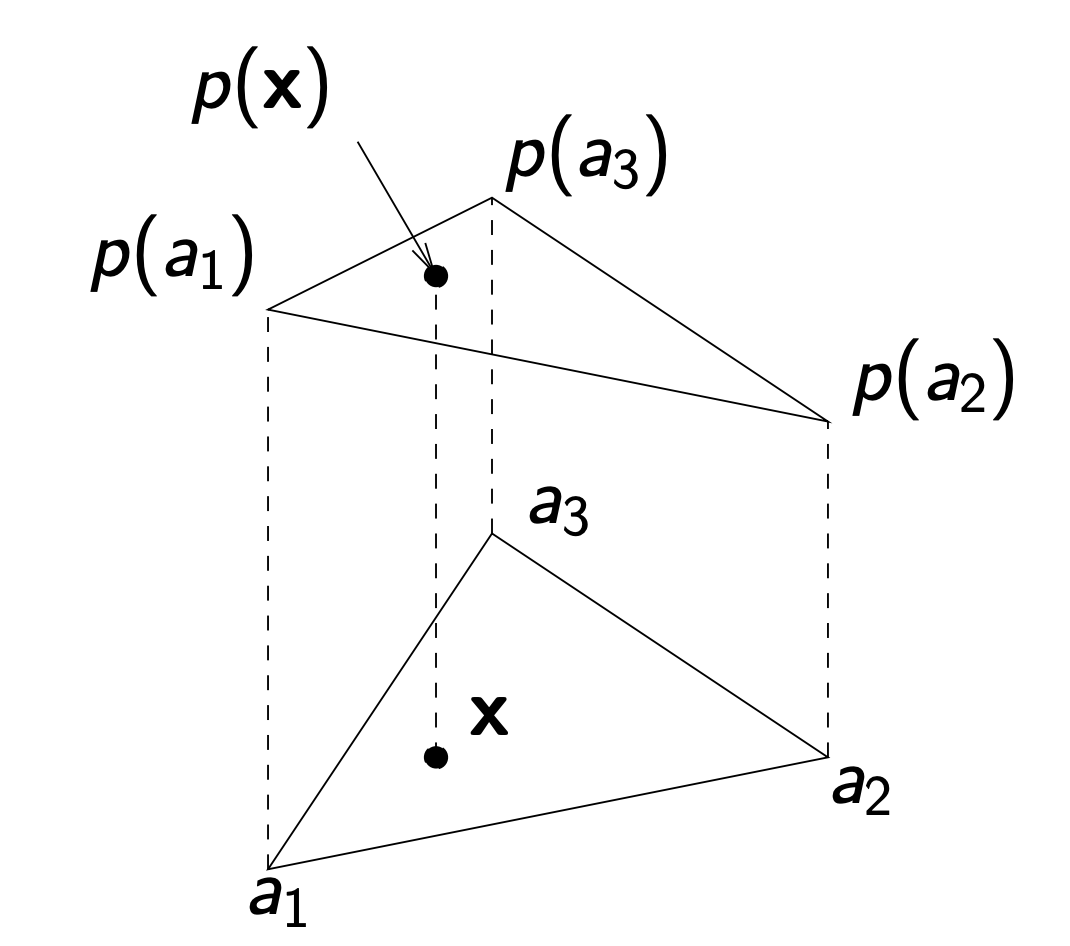
\includegraphics[scale=0.115]{unisolvant.png} 
\end{center}
\end{itemize}
\end{frame}
%%%%%%%%%%%%%%%%%%%%%%%%%%%%%%%%%%%%%%%%%%%%%%%%%%%%%%%

\begin{frame}
\frametitle{Éléments finis de Lagrange}

 \begin{itemize}
 
\item On suppose l'application $F$ injective. Alors si $(\widehat{K}, \widehat{\mathbb{P}}, \widehat{\Sigma})$ est un élément fini de Lagrange, le triplet $(K, \mathbb{P}, \Sigma)$, où $K=F(\widehat{K})$ et où 
on a posé
\begin{equation}
\mathbb{P}=\{p:K\to\mathbb{R};\; p\circ F\,\in \widehat{\mathbb{P}}\},\quad\mbox{ et }\quad\Sigma = F(\widehat{\Sigma})),
\label{transformation}
\end{equation}
est un élément fini de Lagrange.
\item Deux éléments finis de Lagrange $(\widehat{K},\widehat{P},\widehat{\Sigma})$ et $(K, P, \Sigma)$ sont dits affine-équivalents s'il existe une bijection $F$ de $\widehat{K}$ sur $K$ vérifiant \eqref{transformation} ; 
 \end{itemize}
\begin{center}
\begin{tikzpicture}[domain=0:5,scale=0.5]
 \pgfmathsetmacro{\alpha}{0.05}
  \pgfmathsetmacro{\a}{0.5}
  \draw[->] (0,0) -- (5,0)  node[right] {$\xi$};
  \draw[->] (0,0) -- (0,5) node[left] {$\eta$};
 \draw[->] (8,0) -- ++(7,0)  node[right] {$x$};
  \draw[->] (8,0) --++ (0,5) node[left] {$y$};
   \draw[blue,thick,fill=blue!30, fill opacity=0.6](10,2)-- ++(3,-1)-- ++(0,3)-- ++(-3,-2);

\path[fill=gray] (10,2) circle (1.0mm)node[left,below] {$\scriptstyle  a_i$};
\path[fill=gray] (13,1) circle (1.0mm)node[left,below] {$\scriptstyle  a_j$};
\path[fill=gray] (13,4) circle (1.0mm)node[right] {$\scriptstyle  a_k$};


\draw[fill=orange!30, fill opacity=0.6] (0,0) -- ++(3,0) -- ++(-3,3) -- ++(0,-3) ;
\draw (2,0)  node[below] {$\scriptstyle  \widehat{x} =(\xi,\eta)$};
\draw (11,0)  node[below] {\small {\bf x} $\scriptstyle =\,(x,y)$};
  
 \draw [->, >=latex,olive] (1,1.5) arc (120:70:13) ;
\end{tikzpicture}

\end{center}
\end{frame}
%%%%%%%%%%%%%%%%%%%%%%%%%%%%%%%%%%%%%%%%%%%%%%%%%%%%%%%

%\begin{frame}
%\frametitle{Éléments finis de Lagrange}
%
%\begin{theorem}
%Soit$(\widehat{K},\widehat{P},\widehat{\Sigma})$ et $(K, P, \Sigma)$ deux éléments finis de Lagrange équivalents et $F$ une bijection de $\widehat{K}$ sur $K$  vérifiant (4.1-6) et (4.1-7). Si $\widehat{\Pi}$ est l'opérateur de :$\widehat{P}$-interpolation sur $\widehat{\Sigma}$, l'opérateur $\Pi$ de $P$-interpolation sur $\Sigma$ est caractérisé par
%\begin{equation}
%(\Pi v)\circ F = \widehat{\Pi}(v\circ F)
%\end{equation}
%pour toute fonction $v$ définie sur $K$, c'est-à-dire
%\begin{equation}
%\widehat{\Pi v} =\widehat{\Pi} \widehat{v}
%\end{equation}
%\end{theorem}
%
%
%\end{frame}
%%%%%%%%%%%%%%%%%%%%%%%%%%%%%%%%%%%%%%%%%%%%%%%%%%%%%%%

\begin{frame}
\frametitle{Éléments finis simpliciaux}

\begin{center}
\begin{tikzpicture}[domain=0:5,scale=0.3]
 \pgfmathsetmacro{\alpha}{0.05}
  \pgfmathsetmacro{\a}{0.5}
  \draw[orange,->] (-2,2) -- (5,2)  node[right] {$x$};
  \path[fill=gray] (0,2) circle (1.0mm)node[left,below] {$\scriptstyle  a_1$};
  \path[fill=gray] (3,2) circle (1.0mm)node[left,below] {$\scriptstyle  a_2$};
  \draw[blue,thick] (0,2) -- (3,2);
  
 \draw[orange,->] (10,1) -- ++(7,0)  node[right] {$x$};
  \draw[orange,->] (10,1) --++ (0,5) node[left] {$y$};
   \draw[blue,thick,fill=blue!30, fill opacity=0.6](12,3)-- ++(3,-1)-- ++(0,3)-- ++(-3,-2);

\path[fill=gray] (12,3) circle (1.0mm)node[left,below] {$\scriptstyle  a_1$};
\path[fill=gray] (15,2) circle (1.0mm)node[left,below] {$\scriptstyle  a_2$};
\path[fill=gray] (15,5) circle (1.0mm)node[right] {$\scriptstyle  a_3$};

\draw[orange,->] (25,1) --++ (-1.5,-1.5) node[left] {$x$};
 \draw[orange,->] (25,1) -- ++(7,0)  node[right] {$y$};
  \draw[orange,->] (25,1) --++ (0,5) node[left] {$z$};


\path[fill=gray] (27,3) circle (1.0mm)node[left,below] {$\scriptstyle  a_1$};
\path[fill=gray] (30,2) circle (1.0mm)node[left,below] {$\scriptstyle  a_2$};
\path[fill=gray] (32,3) circle (1.0mm)node[right] {$\scriptstyle  a_3$};
\path[fill=gray] (29,6) circle (1.0mm)node[right] {$\scriptstyle  a_4$};
   \draw[blue,thick,fill=blue!30, fill opacity=0.6] (27,3)-- ++(3,-1)-- ++(-1,4)-- ++(-2,-3);
      \draw[blue,thick,fill=blue!20, fill opacity=0.5] (30,2)-- ++(2,1)-- ++(-3,3);
  \draw[blue,dashed] (27,3)--(32,3);
\draw[olive] (1,0)  node[below] {dim 1};
\draw[olive]  (13,0)  node[below] {dim 2};
\draw[olive]  (28,0)  node[below] {dim 2};

\end{tikzpicture}

\end{center}

On considère $n +1$ points $a_j=(a_{ij})_{i=1}^n\in \mathbb{R}^n$, $1\leq j \leq n+1$, non situés dans un même hyperplan, c'est-à-dire tels que la matrice d'ordre $n +1$

\begin{equation}
A=\left(\begin{array}{llll}
a_{11} & a_{12} & \cdots & a_{1,n+1} \\ 
a_{21} & a_{22} & \cdots & a_{2,n+1} \\ 
\vdots& \vdots &  & \vdots \\ 
a_{n1} & a_{n2} & \cdots & a_{n,n+1} \\ 
1 & 1 & \cdots & 1
\end{array}\right)
\end{equation}
soit inversible. On appelle $n$-simplexe $K$ de sommets $a_j$, $1\leq j\leq n+1$,                                                                                                         l'enveloppe convexe des points $a_j$ ; 
%\begin{itemize}
%\item pour $n=2$, $K$ est un triangle.
%\item pour $n = 3$, $K$ est un tétraèdre.
%\end{itemize}
\end{frame}
%%%%%%%%%%%%%%%%%%%%%%%%%%%%%%%%%%%%%%%%%%%%%%%%%%%%%%%

\begin{frame}
\frametitle{Coordonnées barycentriques}
  Tout point $x$ de $\mathbb{R}^n$, de coordonnées cartésiennes $x_i$, $1\leq i\leq n$, est caractérisé par la donnée des $n+ 1$ scalaires ,$\lambda_j=\lambda_j(x)$, $1\leq j \leq n+1$, définis comme solution du système linéaire

\begin{equation}
\left\{\begin{array}{l}
\displaystyle x=\sum_{j=1}^{n+1}\lambda_j(x) a_{j}\\
\displaystyle \sum_{j=1}^{n+1}\lambda_j =1
\end{array}\right.
\Longleftrightarrow
\left\{\begin{array}{l}
\displaystyle \sum_{j=1}^{n+1}a_{ij}\lambda_j =x_i, \quad 1\leq i\leq n\\
\displaystyle \sum_{j=1}^{n+1}\lambda_j =1
\end{array}\right.
\label{systLinBarycentrique}
\end{equation}
Ces scalaires $\lambda_j(x)$ sont  appelés les coordonnées barycentriques du point $x$ par rapport aux $n+ 1$ points 
$a_j$, $1\leq j\leq n+1$. D'après \eqref{systLinBarycentrique}, chacune de ces fonctions coordonnées barycentriques est une fonction affine de $\mathbb{R}^n$ dans $\mathbb{R}$

\end{frame}


%%%%%%%%%%%%%%%%%%%%%%%%%%%%%%%%%%%%%%%%%%%%%%%%%%%%%%%

\begin{frame}
\frametitle{Polynôme d'interpolation en dimension $n$}

Le $n$-simplexe $K$ de sommets $a_j$, $1\leq j\leq n+1$, est caractérisé par
\begin{equation}
K=\{x\in \mathbb{R}^n;\;0\leq \lambda_j(x) \leq 1,\; 1\leq j\leq n+1\}
\end{equation}
Pour tout entier   $k\geq 0$,  on désigne par $\mathbb{P}_k^{(n)}$ l'espace des (fonctions) polynômes de $\mathbb{R}^n$ dans $\mathbb{R}$ de degré inférieur ou égal à $k$:
\begin{equation}
\forall x\in\mathbb{R}^n,\quad p(x)=\sum_{\begin{array}{c} i_1\geq 0,\cdots ,i_n\geq 0\\i_1+\cdots +i_n\leq k \end{array}}\alpha_{i_1,\cdots,i_n}x_1^{i_1}\cdots x_n^{i_n},
\end{equation}
où les $\alpha_{i_1,\cdots,i_n}$  sont des scalaires réels.

  L'espace des polynômes à $n$ variables homogènes de degré $k$ est de dimension 
$\binom {n+k-1}k$, nombre de combinaisons avec répétitions de longueur $k$ formées à partir des éléments d'un ensemble de cardinal $n$. Par conséquent, la dimension de l'espace $\mathbb{P}_k^{(n)}$ est
\begin{equation}
\dim(\mathbb{P}_k^{(n)})=\sum_{l=0}^k \binom {n+l-1}l=\binom {n+k}k=\frac{(n+k)!}{n!k!}
\end{equation}
\end{frame}

%%%%%%%%%%%%%%%%%%%%%%%%%%%%%%%%%%%%%%%%%%%%%%%%%%%%%%%
%%%%%%%%%%%%%%%%%%%%%%%%%%%%%%%%%%%%%%%%%%%%%%%%%%%%%%%

\begin{frame}
\frametitle{Polynôme d'interpolation en dimension 1}

\begin{itemize}
\item $n=1$
\[
\forall x\in\mathbb{R},\quad p(x)=\sum_{i=0}^k\alpha_{i}x^{i},
\]
\[\mathbb{P}_k^{(1)}=vect\{1,x,x^2,\cdots,x^k\},\quad \dim \mathbb{P}_k^{(1)}=k+1\]
En particuler
\[\mathbb{P}_0^{(1)}=vect\{1\}=\mathbb{R} ,\quad \dim \mathbb{P}_0^{(1)}=1\]
\[\mathbb{P}_1^{(1)}=\{ax+b; a\in\mathbb{R}\mbox{ et }b\in\mathbb{R}\},\quad \dim \mathbb{P}_1^{(1)}=2\]
\[\mathbb{P}_2^{(1)}=\{ax^2+bx+c; a,b,c\in\mathbb{R}\},\quad \dim \mathbb{P}_1^{(1)}=3\]
\end{itemize}

\end{frame}

%%%%%%%%%%%%%%%%%%%%%%%%%%%%%%%%%%%%%%%%%%%%%%%%%%%%%%%%%%%%%%%%%%%%%%%%%%%%%%%%%%%%%%%%%%%%%%%%%%%%%%%%%%%%%%

\begin{frame}
\frametitle{Polynôme d'interpolation en dimension 2}

\begin{itemize}
\item $n=2$
\[
\forall (x,y)\in\mathbb{R},\quad p(x,y)=\sum_{0\leq i+j\leq k}\alpha_{ij}x^{i}y^j,
\]
\[\mathbb{P}_k^{(2)}=vect\{x^iy^j;\; 0\leq i+j \leq k\}, \quad \dim \mathbb{P}_k^{(2)}=\frac{(k+1)(k+2)}{2}\]
En particuler
\[\mathbb{P}_0^{(2)}=vect\{1\}=\mathbb{R} ,\quad \dim \mathbb{P}_0^{(2)}=1\]
\[\mathbb{P}_1^{(2)}=vect\{1,x,y\},\quad \dim \mathbb{P}_1^{(2)}=3\]
\[\mathbb{P}_2^{(2)}=vect\{1,x,x^2,y,y^2,xy\},\quad \dim \mathbb{P}_2^{(2)}=6\]
\end{itemize}

\end{frame}

%%%%%%%%%%%%%%%%%%%%%%%%%%%%%%%%%%%%%%%%%%%%%%%%%%%%%%%
%%%%%%%%%%%%%%%%%%%%%%%%%%%%%%%%%%%%%%%%%%%%%%%

\begin{frame}
\frametitle{Polynôme d'interpolation en dimension 3}

\begin{itemize}
\item $n=3$
\[
\forall (x,y,z)\in\mathbb{R},\quad p(x,y,z)=\sum_{0\leq p+q+r\leq k}\alpha_{pqr}x^{p}y^qz^r,
\]
\[\mathbb{P}_k^{(3)}=vect\{x^{p}y^qz^r; 0\leq p+q+r \leq k\}, \dim \mathbb{P}_k^{(3)}=\frac{(k+1)(k+2)(k+3)}{6}\]
En particuler
\[\mathbb{P}_0^{(3)}=vect\{1\}=\mathbb{R} ,\quad \dim \mathbb{P}_0^{(3)}=1\]
\[\mathbb{P}_1^{(3)}=vect\{1,x,y,z\},\quad \dim \mathbb{P}_1^{(3)}=4\]
\[\mathbb{P}_2^{(3)}=vect\{1,x,x^2,y,y^2,z,z^2,xy,xz,yz\},\quad \dim \mathbb{P}_2^{(3)}=10\]
\end{itemize}

\end{frame}

%%%%%%%%%%%%%%%%%%%%%%%%%%%%%%%%%%%%%%%%%%%%%%%%%%%%%%%
\begin{frame}
\frametitle{Espace de polynômes d'interpolation}

\begin{itemize}
\item $\mathbb{P}_k^{(1)}=vect\{1,x,x^2,\cdots,x^k\}$, $\dim \mathbb{P}_k^{(1)}=k+1$.
\item $\mathbb{P}_k^{(2)}=vect\{x^iy^j;\; 0\leq i+j \leq k\}$, $\dim \mathbb{P}_k^{(2)}=\frac{(k+1)(k+2)}{2}$.
\item $\mathbb{P}_k^{(3)}=vect\{x^iy^jx^k;\; 0\leq i+j+k \leq k\}$, $\dim \mathbb{P}_k^{(2)}=\frac{(k+1)(k+2)(k+3)}{6}$.
\end{itemize}


\hrule


\begin{itemize}
\item $\mathbb{Q}_k^{(1)}=\mathbb{P}_k^{(1)}$.
\item $\mathbb{Q}_k^{(2)}=vect\{x^iy^j;\; 0\leq i,j \leq k\}$, $\dim \mathbb{Q}_k^{(2)}=(k+1)^2$.
\item $\mathbb{Q}_k^{(3)}=vect\{x^iy^jx^k;\; 0\leq i,j,k \leq k\}$, $\dim \mathbb{Q}_k^{(2)}=(k+1)^3$.
\end{itemize}
\end{frame}

%%%%%%%%%%%%%%%%%%%%%%%%%%%%%%%%%%%%%%%%%%%%%%%%%%%%%%%
\begin{frame}
\frametitle{Treillis principal d'ordre $k$}

  On définit enfin, pour tout entier $k$ le treillis d'ordre $k$ du $n$-simplexe $K$ comme étant l'ensemble de points de $\mathbb{R}^n$ défini  par
\begin{equation}
\Sigma_k^{(n)}=\left\{x\in\mathbb{R}^n;\;\lambda_j(x)\in\{0,\frac 1k,\cdots,\frac{k-1}{k},1\}, \;1\leq j\leq n+1\right\}
\end{equation}
  %Pour k=0, on posera
\begin{equation}
\Sigma_0^{(n)}=\left\{x\in\mathbb{R}^n;\;\lambda_j(x)=\frac{1}{n+1}, \;1\leq j\leq n+1\right\}
\end{equation}
\begin{center}
 \begin{tikzpicture}[scale=0.25]
 \draw (-7,0)--++(6,0);
 \path[fill=gray] (-7,0) circle (1.8mm);
 \path[fill=gray] (-5,0) circle (1.8mm);
 \path[fill=gray] (-3,0) circle (1.8mm);
 \path[fill=gray] (-1,0) circle (1.8mm);
 \draw (-7,1.5)--++(6,0);
 \path[fill=gray] (-7,1.5) circle (1.8mm);
 \path[fill=gray] (-4,1.5) circle (1.8mm);
 \path[fill=gray] (-1,1.5) circle (1.8mm);
 \draw (-7,3)--++(6,0);
 \path[fill=gray] (-7,3) circle (1.8mm);
 %\path[fill=orange] (-4,0) circle (1.8mm);
 \path[fill=gray] (-1,3) circle (1.8mm);
  \draw (-7,4.5)--++(6,0);
 %\path[fill=gray] (-7,6) circle (1.8mm);
 \path[fill=gray] (-4,4.5) circle (1.8mm);
 %\path[fill=gray] (-1,6) circle (1.8mm);
 
  \draw (0,0)--++(4,1)--++(-1,4)--++(-3,-5);
  \path[fill=orange] (2.33,2) circle (1.8mm);
  \draw (5,0)--++(4,1)--++(-1,4)--++(-3,-5);
  \path[fill=orange] (5,0) circle (1.8mm);
   \path[fill=orange] (9,1) circle (1.8mm);
   \path[fill=orange] (8,5) circle (1.8mm);
  
  \draw (10,0)--++(4,1)--++(-1,4)--++(-3,-5);
  \path[fill=orange] (10,0) circle (1.8mm);
   \path[fill=orange] (14,1) circle (1.8mm);
   \path[fill=orange] (13,5) circle (1.8mm);
   
    \path[fill=orange] (10+2,0.5) circle (1.8mm);
   \path[fill=orange] (10+3.5,3) circle (1.8mm);
   \path[fill=orange] (10+1.5,2.5) circle (1.8mm);
  \draw (15,0)--++(4,1)--++(-1,4)--++(-3,-5);
   \path[fill=orange] (15,0) circle (1.8mm);
   \path[fill=orange] (19,1) circle (1.8mm);
   \path[fill=orange] (18,5) circle (1.8mm);
   
   \path[fill=orange] (15+1.33,0.33) circle (1.8mm);
   \path[fill=orange] (15+2.66,0.66) circle (1.8mm);
   \path[fill=orange] (15+3.67,2) circle (1.8mm);
   \path[fill=orange] (15+3.33,3.66) circle (1.8mm);
   \path[fill=orange] (15+2,3.33) circle (1.8mm);
   \path[fill=orange] (15+1.,1.66) circle (1.8mm);
 \path[fill=black] (0,0) circle (0.3mm) [fill=gray];
 \path[fill=orange] (15+2.33,2) circle (1.8mm);
 %%%%%%%%%%%%%%%%%%%%%%%%%%%%%%%%%%%
 \draw (20,0)--++(6,1)--++(-2,5)--++(-4,-6);
 \draw[dotted] (20,0)--++(2.5,2)--++(3.5,-1);
 \draw [dotted] (20,0)--++(2.5,2)--++(1.5,4);
 \path[fill=black] (20+3.125,2.25) circle (1.8mm);
 
 \draw (27,0)--++(6,1)--++(-2,5)--++(-4,-6);
 \draw[dotted] (27,0)--++(2.5,2)--++(3.5,-1);
 \draw [dotted] (27,0)--++(2.5,2)--++(1.5,4);
 \path[fill=blue] (27,0) circle (1.8mm);
 \path[fill=blue] (27+6,1) circle (1.8mm);
 \path[fill=blue] (27+4,6) circle (1.8mm);
 \path[fill=blue] (27+2.5,2) circle (1.8mm);
 
 \draw (34,0)--++(6,1)--++(-2,5)--++(-4,-6);
 \draw[dotted] (34,0)--++(2.5,2)--++(3.5,-1);
 \draw [dotted] (34,0)--++(2.5,2)--++(1.5,4);
 \path[fill=blue] (34,0) circle (1.8mm);
 \path[fill=blue] (34+6,1) circle (1.8mm);
 \path[fill=blue] (34+4,6) circle (1.8mm);
 \path[fill=blue] (34+2.5,2) circle (1.8mm);
 \path[fill=blue] (34+3,0.5) circle (1.8mm);
 \path[fill=blue] (34+5,3.5) circle (1.8mm);
 \path[fill=blue] (34+2,3) circle (1.8mm);
 \path[fill=blue] (34+1.25,1) circle (1.8mm);
 \path[fill=blue] (34+4.25,1.5) circle (1.8mm);
 \path[fill=blue] (34+3.25,4) circle (1.8mm);


\end{tikzpicture}
 \end{center}
En tenant compte de $\lambda_{n+1}=1-\sum_{j=1}^n\lambda_j$, on vérifie que le cardinal de l'ensemble $\Sigma_k^{(n)}$ est le nombre de combinaisons avec   répétitions de longueur $k$ formées à partir des éléments de $\{0,\cdots,n\}$                                                                                                                                         d'où 
\begin{equation}
\mbox{card}(\Sigma_k^{(n)})=\binom {(n+1)+k-1}k=\binom {n+k}k=\frac{(n+k)!}{n!k!}
\end{equation}
\end{frame}

%%%%%%%%%%%%%%%%%%%%%%%%%%%%%%%%%%%%%%%%%%%%%%%%%%%%%%%
%%%%%%%%%%%%%%%%%%%%%%%%%%%%%%%%%%%%%%%%%%%%%%%%%%%%%%%
\begin{frame}
\frametitle{Treillis principal d'ordre $k$ en dimension 1}
\begin{equation}
\Sigma_k^{(1)}=\left\{x\in\mathbb{R};\;\lambda_j(x)\in\{0,\frac 1k,\cdots,\frac{k-1}{k},1\}, \;1\leq j\leq 2\right\}
\end{equation}
  %Pour k=0, on posera
\begin{equation}
\Sigma_0^{(1)}=\left\{x\in\mathbb{R};\;\lambda_1(x)=\lambda_2(x)=\frac{1}{2}\right\}=\left\{x=\frac{a_1+a_2}{2}=a_0\right\}
\end{equation}
\begin{center}
 \begin{tikzpicture}[scale=0.25]
 \draw (-7,0)--++(6,0)node[right]{$\scriptstyle  k=3$};
 \path[fill=orange] (-7,0) circle (1.8mm);
 \path[fill=orange] (-5,0) circle (1.8mm);
 \path[fill=orange] (-3,0) circle (1.8mm);
 \path[fill=orange] (-1,0) circle (1.8mm);
 \draw (-7,1.5)--++(6,0)node[right]{$\scriptstyle  k=2$};
 \path[fill=orange] (-7,1.5) circle (1.8mm);
 \path[fill=orange] (-4,1.5) circle (1.8mm);
 \path[fill=orange] (-1,1.5) circle (1.8mm);
 \draw (-7,3)--++(6,0)node[right]{$\scriptstyle  k=1$};
 \path[fill=orange] (-7,3) circle (1.8mm);
 %\path[fill=orange] (-4,0) circle (1.8mm);
 \path[fill=orange] (-1,3) circle (1.8mm);
  \draw (-7,4.5)--++(6,0)node[right]{$\scriptstyle  k=0$};
 %\path[fill=orange] (-7,6) circle (1.8mm);
 \path[fill=orange] (-4,4.5) circle (1.8mm);
 %\path[fill=gray] (-1,6) circle (1.8mm);
 
 %%%%%%%%%%%%%%%%%%%%%%%%%%%%%%%%%%%
 
\end{tikzpicture}
 \end{center}
 En particulier
 \begin{equation}
\Sigma_1^{(1)}=\left\{ x=\lambda_1 a_1+\lambda_2 a_2; \;\lambda_j\in\{0,1\}\right\}=\{a_1,a_2\}
\end{equation}
 \begin{equation}
\Sigma_2^{(1)}=\left\{ x=\lambda_1 a_1+\lambda_2 a_2; \;\lambda_j\in\{0,\frac 12,1\}\right\}=\{a_1,a_2,a_0\}
\end{equation}
 \begin{equation}
\Sigma_3^{(1)}=\left\{ x=\lambda_1 a_1+\lambda_2 a_2; \;\lambda_j\in\{0,\frac 13,\frac 23,1\}\right\}=\{a_1,a_2,a_{112},a_{122}\}
\end{equation}

\end{frame}

%%%%%%%%%%%%%%%%%%%%%%%%%%%%%%%%%%%%%%%%%%%%%%%%%%%%%%%
%%%%%%%%%%%%%%%%%%%%%%%%%%%%%%%%%%%%%%%%%%%%%%%%%%%%%%%
\begin{frame}
\frametitle{Treillis principal d'ordre $k$ en dimension 2}
\begin{equation}
\Sigma_k^{(2)}=\left\{x\in\mathbb{R}^2;\;\lambda_j(x)\in\{0,\frac 1k,\cdots,\frac{k-1}{k},1\}, \;1\leq j\leq 3\right\}
\end{equation}
  %Pour k=0, on posera
\begin{equation}
\Sigma_0^{(2)}=\left\{x\in\mathbb{R}^2;\;\lambda_1=\lambda_2=\lambda_3=\frac{1}{3}\right\}=\left\{x=\frac{a_1+a_2+a_3}{3}=a_0\right\}
\end{equation}
\begin{center}
 \begin{tikzpicture}[scale=0.25]
   \draw (0,0)--++(4,1)--++(-1,4)--++(-3,-5);
  \path[fill=orange] (2.33,2) circle (1.8mm);
  \draw (5,0)--++(4,1)--++(-1,4)--++(-3,-5);
  \path[fill=orange] (5,0) circle (1.8mm);
   \path[fill=orange] (9,1) circle (1.8mm);
   \path[fill=orange] (8,5) circle (1.8mm);
  
  \draw (10,0)--++(4,1)--++(-1,4)--++(-3,-5);
  \path[fill=orange] (10,0) circle (1.8mm);
   \path[fill=orange] (14,1) circle (1.8mm);
   \path[fill=orange] (13,5) circle (1.8mm);
   
    \path[fill=orange] (10+2,0.5) circle (1.8mm);
   \path[fill=orange] (10+3.5,3) circle (1.8mm);
   \path[fill=orange] (10+1.5,2.5) circle (1.8mm);
  \draw (15,0)--++(4,1)--++(-1,4)--++(-3,-5);
   \path[fill=orange] (15,0) circle (1.8mm);
   \path[fill=orange] (19,1) circle (1.8mm);
   \path[fill=orange] (18,5) circle (1.8mm);
   
   \path[fill=orange] (15+1.33,0.33) circle (1.8mm);
   \path[fill=orange] (15+2.66,0.66) circle (1.8mm);
   \path[fill=orange] (15+3.67,2) circle (1.8mm);
   \path[fill=orange] (15+3.33,3.66) circle (1.8mm);
   \path[fill=orange] (15+2,3.33) circle (1.8mm);
   \path[fill=orange] (15+1.,1.66) circle (1.8mm);
 \path[fill=black] (0,0) circle (0.3mm) [fill=gray];
 \path[fill=orange] (15+2.33,2) circle (1.8mm);
 %%%%%%%%%%%%%%%%%%%%%%%%%%%%%%%%%%%
 
\end{tikzpicture}
 \end{center}
 \begin{equation}
\Sigma_1^{(2)}=\left\{ x=\lambda_1 a_1+\lambda_2 a_2+\lambda_3 a_3; \;\lambda_j\in\{0,1\}\right\}=\{a_1,a_2,a_3\}
\end{equation}
 \[
\Sigma_2^{(2)}=\left\{ x=\lambda_1 a_1+\lambda_2 a_2+\lambda_3 a_3; \;\lambda_j\in\{0,\frac 12,1\}\right\}=\{a_1,a_2,a_3,a_{12},a_{13},a_{23}\}
\]
 \[\begin{array}{rcl}
 \Sigma_3^{(2)}&=&\displaystyle \left\{ x=\lambda_1 a_1+\lambda_2 a_2+\lambda_3 a_3; \;\lambda_j\in\{0,\frac 13,\frac 23,1\}\right\}\\
 &=&\{a_1,a_2,a_3,a_{112},a_{122},a_{113},a_{133},a_{223},a_{233},a_0\}
 \end{array}\]


\end{frame}

%%%%%%%%%%%%%%%%%%%%%%%%%%%%%%%%%%%%%%%%%%%%%%%%%%%%%%%
%%%%%%%%%%%%%%%%%%%%%%%%%%%%%%%%%%%%%%%%%%%%%%%%%%%%%%%
\begin{frame}
\frametitle{Treillis principal d'ordre $k$ en dimension 3}
\[
\Sigma_k^{(3)}=\left\{x\in\mathbb{R}^3;\;\lambda_j(x)\in\{0,\frac 1k,\cdots,\frac{k-1}{k},1\}, \;1\leq j\leq 4\right\}
\]
  %Pour k=0, on posera
\[
\Sigma_0^{(3)}=\left\{x\in\mathbb{R}^3;\;\lambda_1=\lambda_2=\lambda_3=\lambda_4=\frac{1}{4}\right\}=\left\{\frac{a_1+a_2+a_3+a_4}{4}=a_0\right\}
\]
\begin{center}
 \begin{tikzpicture}[scale=0.25]
 \draw (20,0)--++(6,1)--++(-2,5)--++(-4,-6);
 \draw[dotted] (20,0)--++(2.5,2)--++(3.5,-1);
 \draw [dotted] (20,0)--++(2.5,2)--++(1.5,4);
 \path[fill=orange] (20+3.125,2.25) circle (1.8mm);
 
 \draw (27,0)--++(6,1)--++(-2,5)--++(-4,-6);
 \draw[dotted] (27,0)--++(2.5,2)--++(3.5,-1);
 \draw [dotted] (27,0)--++(2.5,2)--++(1.5,4);
 \path[fill=orange] (27,0) circle (1.8mm);
 \path[fill=orange] (27+6,1) circle (1.8mm);
 \path[fill=orange] (27+4,6) circle (1.8mm);
 \path[fill=orange] (27+2.5,2) circle (1.8mm);
 
 \draw (34,0)--++(6,1)--++(-2,5)--++(-4,-6);
 \draw[dotted] (34,0)--++(2.5,2)--++(3.5,-1);
 \draw [dotted] (34,0)--++(2.5,2)--++(1.5,4);
 \path[fill=orange] (34,0) circle (1.8mm);
 \path[fill=orange] (34+6,1) circle (1.8mm);
 \path[fill=orange] (34+4,6) circle (1.8mm);
 \path[fill=orange] (34+2.5,2) circle (1.8mm);
 \path[fill=orange] (34+3,0.5) circle (1.8mm);
 \path[fill=orange] (34+5,3.5) circle (1.8mm);
 \path[fill=orange] (34+2,3) circle (1.8mm);
 \path[fill=orange] (34+1.25,1) circle (1.8mm);
 \path[fill=orange] (34+4.25,1.5) circle (1.8mm);
 \path[fill=orange] (34+3.25,4) circle (1.8mm);

 %%%%%%%%%%%%%%%%%%%%%%%%%%%%%%%%%%%
 
\end{tikzpicture}
 \end{center}
 \[
\Sigma_1^{(3)}=\left\{ x=\lambda_1 a_1+\lambda_2 a_2+\lambda_3 a_3+\lambda_4 a_4; \;\lambda_j\in\{0,1\}\right\}=\{a_1,a_2,a_3,a_4\}
\]
 \[\begin{array}{rcl}
 \Sigma_2^{(3)}&=&\displaystyle \left\{ x=\lambda_1 a_1+\lambda_2 a_2+\lambda_3 a_3+\lambda_4 a_4; \;\lambda_j\in\{0,\frac 12,1\}\right\}\\
 &=&\{a_1,a_2,a_3,a_{12},a_{13},a_{14},a_{23},a_{24},a_{34},a_0\}
 \end{array}\]


\end{frame}

%%%%%%%%%%%%%%%%%%%%%%%%%%%%%%%%%%%%%%%%%%%%%%%%%%%%%%%

\begin{frame}
\frametitle{Élément fini $n$-simplexe}
\begin{itemize}
\item Pour tout entier $k\geq 0$, l'ensemble $\Sigma_k^{(n)}$ , est $P_k^{(n)}$-unisolvant.
 \item Pour tout $n$-simplexe $K^{(n)}$ de $\mathbb{R}^n$ et pour tout entier   $k\geq 0$,    l'élément fini $(K^{(n)}, P_k^{(n)}, \Sigma_k^{(n)})$, où $\Sigma_k^{(n)}$ est le treillis principal d'ordre $k$ de $K^{(n)}$, est appelé $n$-simplexe de type ($k$).
\item Pour tout entier $k\geq 0$, deux éléments finis $n$-simplexes de type ($k$) sont affine-équivalents.

\end{itemize}

\begin{center}
\begin{tikzpicture}[domain=0:5,scale=0.4]
 \pgfmathsetmacro{\alpha}{0.05}
  \pgfmathsetmacro{\a}{0.5}
  \draw[->] (0,0) -- (5,0)  node[right] {$\xi$};
  \draw[->] (0,0) -- (0,5) node[left] {$\eta$};
 \draw[->] (8,0) -- ++(7,0)  node[right] {$x$};
  \draw[->] (8,0) --++ (0,5) node[left] {$y$};
   \draw[blue,thick,fill=blue!30, fill opacity=0.6](10,2)-- ++(3,-1)-- ++(0,3)-- ++(-3,-2);

\path[fill=gray] (10,2) circle (1.0mm)node[left,below] {$\scriptstyle  a_i$};
\path[fill=gray] (13,1) circle (1.0mm)node[left,below] {$\scriptstyle  a_j$};
\path[fill=gray] (13,4) circle (1.0mm)node[right] {$\scriptstyle  a_k$};


\draw[fill=orange!30, fill opacity=0.6] (0,0) -- ++(3,0) -- ++(-3,3) -- ++(0,-3) ;
\draw (2,0)  node[below] {$\scriptstyle  \widehat{x} =(\xi,\eta)$};
\draw (11,0)  node[below] {\small {\bf x} $\scriptstyle =\,(x,y)$};
  
 \draw [->, >=latex,olive] (1,1.5) arc (120:70:13) ;
\end{tikzpicture}

\end{center}

 Il suffira donc d'étudier les propriétés d'un $n$-simplexe de type ($k$) particulier $(\widehat{K_k}^{(n)} , \widehat{P_k}^{(n)} , \widehat{\Sigma}^{(n)}_k)$  appelé $n$-simplexe de référence.
\end{frame}
%%%%%%%%%%%%%%%%%%%%%%%%%%%%%%%%%%%%%%%%%%%%%%%%%%%%%%%

\begin{frame}
\frametitle{Élément fini $n$-simplexe de référence}

On choisit pour $\widehat{K}$ le n-simplexe unité de sommets 
$\hat{a}_1= (1 , 0, \cdots, 0)$ , $\hat{a}_2= (0,1 , 0, \cdots, 0)$, ... $\hat{a}_n= (0 , \cdots, 0,1)$, $\hat{a}_{n+1}= (0 , 0, \cdots, 0)$. Dans ce cas, les coordonnées barycentriques sont
\begin{equation}
\hat{\lambda}_i(\hat{x})=\hat{x}_i,\; 1\leq i\leq n;\quad \hat{\lambda}_{n+1}=1-\sum_{i=1}^n\hat{\lambda}_i,
\end{equation}
       Considérons un peu plus en détail les éléments finis $(K, P, \Sigma)$ $n$-simplexes de 
type ($k$) les plus couramment utilisés en pratique.

%Lorsque $n=1$, $K$ est le segment d'extrémités $a_1$, $a_2$. 
On pose
\[\begin{array}{lcll}
a_{0}&=&\frac{1}{2}(a_1+a_2),&\mbox{ milieu du segment }\\
a_{0}&=&\displaystyle \frac{1}{n+1}\sum_{i=1}^{n+1}a_i,&\mbox{ centre de gravité }\\
a_{iij}&=&\frac{1}{3}(2a_i+a_j), & \mbox{ au tiers du segment }\\
a_{ijj}&=&\frac{1}{3}(a_i+2a_j), &  \mbox{ au deux-tiers du segment }
\end{array}
\]

\end{frame}
%%%%%%%%%%%%%%%%%%%%%%%%%%%%%%%%%%%%%%%%%%%%%%%%%%%%%%%
\begin{frame}
\frametitle{Élément fini segment}

\begin{itemize}
\item  \fbox{$n=1$, $k=0$}  Le segment de type (0) correspond à 
\[(K,P,\Sigma)=([0,1],\;\mathbb{P}_0^{(1)}=\mathbb{R},\;\Sigma_0^{(1)} = \{a_0\})\]
La fonction de base est $\varphi(\xi)=1$
\begin{tikzpicture}[scale=1]
\draw  [very thin, gray] [->]  (-0.2,0) -- (1.2,0); 
\draw  [very thin, gray] [->] (0,-0.2) -- (0,1.2);
\draw  [line width=1pt] (0,0) -- (1,0);
\draw  [dashed] (0.5,0) -- (0.5,1);
\node [blue] at (0.5,0) {$\bullet$};
%\node at (0.5,-0.5) {$\scriptstyle  p_1(\xi)=1$};
\draw [orange,domain=0:1] plot(\x,1);
\node [orange] at (-0.1,1) {$\scriptstyle  1$};
\end{tikzpicture} 
\item  \fbox{$n=1$, $k=1$}  Le segment de type (1) correspond à 
\[(K,P,\Sigma)=([0,1],\;\mathbb{P}_1^{(1)}=\mathbb{R}_1[X],\;\Sigma_1^{(1)} = \{a_1=1,a_2=0\})\]

Les fonctions de base sont les fonctions coordonnées barycentriques:
\[\varphi_1 = \lambda_1=\xi,\quad   \varphi_2 = \lambda_2=1-\xi\]


  	\begin{center}
  	\begin{tabular}{cc}
  	\begin{tikzpicture}[scale=1]
\draw  [very thin, gray] [->]  (-0.2,0) -- (1.2,0); 
\draw  [very thin, gray] [->] (0,-0.2) -- (0,1.2);
\draw  [line width=1pt] (0,0) -- (1,0);
\draw  [dashed] (1,0) -- (1,1);
\node [blue] at (0,0) {$\bullet$};
\node [blue] at (1,0) {$\bullet$};
\node at (0.5,-0.5) {$\scriptstyle \varphi_1(\xi)=\xi$};
\draw [orange,domain=0:1] plot(\x,\x);
\end{tikzpicture} 
 &
 \begin{tikzpicture}[scale=1]
\draw  [very thin, gray] [->]  (-0.2,0) -- (1.2,0); 
\draw  [very thin, gray] [->] (0,-0.2) -- (0,1.2);
\draw  [line width=1pt] (0,0) -- (1,0);
\draw  [dashed] (0,0) -- (0,1);
\node [blue] at (0,0) {$\bullet$};
\node [blue] at (1,0) {$\bullet$};
\node at (0.5,-0.5) {$\scriptstyle  \varphi_2(\xi)=1-\xi$};
\draw [orange,domain=0:1] plot(\x,1-\x);

\end{tikzpicture} 
\end{tabular}
  	\end{center}
  	

  \end{itemize}	
 \end{frame}  

\begin{frame}
\frametitle{Élément fini segment}

\begin{itemize}
\item   \fbox{$n=1$, $k=1$}, le segment de type (2) correspond à
    \[\mathbb{P}=\mathbb{P}_2,\quad \Sigma=\Sigma_2 = \{a_1,a_{12},a_2\}\]
Les fonctions de base sont les fonctions
\[\left\{\begin{array}{l}
\varphi_i=\lambda_i(2\lambda_i-1), \quad i=1,2 \\
\varphi_{12}=4\lambda_1\lambda_2
\end{array}\right.
\]
\[\varphi_1(\xi)=\xi(2\xi-1),\quad \varphi_2(\xi)=(1-\xi)(2(1-\xi)-1)=(1-\xi)(1-2\xi)\]
\end{itemize}
  	\begin{center}
  	\begin{tabular}{ccc}
  	  \begin{tikzpicture}[scale=1]
\draw  [very thin, gray] [->]  (-0.2,0) -- (1.2,0); 
\draw  [very thin, gray] [->] (0,-0.2) -- (0,1.2);
\draw  [line width=1pt] (0,0) -- (1,0);
\draw  [dashed] (1,0) -- (1,1);
\node [blue] at (0,0) {$\bullet$};
\node [blue] at (0.5,0) {$\bullet$};
\node [blue] at (1,0) {$\bullet$};
\node at (0.5,-0.5) {$\scriptstyle  \varphi_1= \xi(2\xi-1)$};
\draw [orange,domain=0:1] plot(\x,{\x*(2*\x-1)});

\end{tikzpicture} 
&
  \begin{tikzpicture}[scale=1]
\draw  [very thin, gray] [->]  (-0.2,0) -- (1.2,0); 
\draw  [very thin, gray] [->] (0,-0.2) -- (0,1.2);
\draw  [line width=1pt] (0,0) -- (1,0);
\node [blue] at (0,0) {$\bullet$};
\node [blue] at (0.5,0) {$\bullet$};
\node [blue] at (1,0) {$\bullet$};
\node at (0.5,-0.5) {$\scriptstyle  \varphi_{12}=4\xi(1-\xi) $};
\draw [orange,domain=0:1] plot(\x,{4*\x*(1-\x)});

\end{tikzpicture} 
&
 \begin{tikzpicture}[scale=1]
\draw  [very thin, gray] [->]  (-0.2,0) -- (1.2,0); 
\draw  [very thin, gray] [->] (0,-0.2) -- (0,1.2);
\draw  [line width=1pt] (0,0) -- (1,0);
\draw  [dashed] (0,0) -- (0,1);
\node [blue] at (0,0) {$\bullet$};
\node [blue] at (0.5,0) {$\bullet$};
\node [blue] at (1,0) {$\bullet$};
\node at (0.5,-0.5) {$\scriptstyle \varphi_2=(1-\xi)(1-2\xi) $};
\draw [orange,domain=0:1] plot(\x,{(2*\x-1)*(\x-1)});
%\caption{$ p_1=(1-\xi)(1-2\xi) $}
\end{tikzpicture} 

\end{tabular}
  	\end{center}
	

\end{frame}
%%%%%%%%%%%%%%%%%%%%%%%%%%%%%%%%%%%%%%%%%%%%%%%%%%%%%%%

\begin{frame}
\frametitle{Éléments finis triangles ($n=2$)}

\begin{itemize}
\item Lorsque $n=2$, $K$ est le triangle de sommets $a_1$, $a_2$ et $a_3$. On pose
\[\begin{array}{ll}
a_0=\frac{1}{3}(a_1+a_2+a_3)&\mbox{centre de gravité de }K\\
a_{ij}=\frac{1}{2}(a_i+a_j),&\mbox{milieu du côté }[a_i,a_j] \\
a_{iij}=\frac{1}{3}(2a_i+a_j), &  a_{iij} \mbox{ et } a_{jji} \mbox{ aux tiers et deux-tiers du côté }[a_ia_j].
\end{array}
\]
\begin{center}
\begin{tikzpicture}[domain=0:5,scale=0.5]
 \pgfmathsetmacro{\alpha}{0.05}
  \pgfmathsetmacro{\a}{0.5}
  \draw[->] (0,0) -- (5,0)  node[right] {$\xi$};
  \draw[->] (0,0) -- (0,5) node[left] {$\eta$};
  \draw (3,0)  node[above right] {$\scriptstyle  \widehat{a}_1$};
  \draw (0,3)  node[above right] {$\scriptstyle  \widehat{a}_2$};
  \draw (0,0)  node[above left] {$\scriptstyle  \widehat{a}_3$};
  \draw (0.8,1.5)  node {$\scriptstyle  \widehat{x}$};
  \draw (12.2,2.4)  node {$\scriptstyle  x$};
 \draw[->] (8,0) -- ++(7,0)  node[right] {$x$};
  \draw[->] (8,0) --++ (0,5) node[left] {$y$};
   \draw[blue,thick,fill=blue!30, fill opacity=0.6](10,2)-- ++(3,-1)-- ++(0,3)-- ++(-3,-2);

\path[fill=gray] (10,2) circle (1.0mm)node[left,below] {$\scriptstyle  a_3$};
\path[fill=gray] (13,1) circle (1.0mm)node[left,below] {$\scriptstyle  a_1$};
\path[fill=gray] (13,4) circle (1.0mm)node[right] {$\scriptstyle  a_2$};


\draw[fill=orange!30, fill opacity=0.6] (0,0) -- ++(3,0) -- ++(-3,3) -- ++(0,-3) ;
\draw (2,-0.5)  node[below] {$\scriptstyle  \widehat{x} =\lambda_1\widehat{a}_1+\lambda_2\widehat{a}_2+\lambda_3\widehat{a}_3$};
\draw (11,-0.5)  node[below] {$\scriptstyle  x =\lambda_1 a_1+\lambda_2 a_2+\lambda_3 a_3$};
 \draw [->, >=latex,olive] (1,1.5) arc (120:70:13) ;
\end{tikzpicture}

\end{center}

\end{itemize}
\end{frame}

%%%%%%%%%%%%%%%%%%%%%%%%%%%%%%%%%%%%%%%%%%%%%%%%%%%%%%%

\begin{frame}
\frametitle{Éléments finis triangles de type (0)}

\begin{itemize}

\item  Pour $k=0$, le triangle de type (0) correspond à
    \[ \mathbb{P}=\mathbb{P}_0^{(2)}=\mathbb{R}, \quad \Sigma=\Sigma_0^{(2)} = \{a_0\}\]
La fonction de base est la fonction constante définie par
\[\forall x\in K,\quad \varphi_0(x)=1\]
\begin{center}
\begin{tikzpicture}[scale=0.5]
  \draw[->] (0,0) -- (6,-2) node[right] {$x$};
  \draw[->] (0,0) -- (7.2,2.7) node[right] {$y$};
  \draw[->] (0,0) -- (0,4) node[left] {$z$};
  \draw[line width=1pt] (0,0)--(4.5,-1.5)--(6,2.25)--(0,0);
  \path[fill=orange] (3.5,0.15) circle (1.8mm);
   %\path[fill=orange] (4.5,-1.5) circle (1.8mm);
   %\path[fill=orange] (6,2.25) circle (1.8mm);
   
   \draw[fill=gray!20]  (0,2)--(4.5,-1.5+2)--(6,4.25)--(0,2);
  \draw  [dashed,->] (3.5,0.15) -- ++(0,2);
\end{tikzpicture}
\end{center}

\end{itemize}
\end{frame}
%%%%%%%%%%%%%%%%%%%%%%%%%%%%%%%%%%%%%%%%%%%%%%%%%%%

\begin{frame}
\frametitle{Éléments finis triangles de type (1)}

\begin{itemize}
\item  Pour $k= 1$, le triangle de type (1) est obtenu pour
    \[\mathbb{P}=\mathbb{P}_1^{(2)}=\{ax+by+c;\;(a,b,c)\in\mathbb{R}^3\} ,\quad \Sigma=\Sigma_1^{(2)}  = \{a_i\}_{1\leq i\leq 3}\]
Les fonctions de base sont les fonctions coordonnées barycentriques par rapport à $(a_1, a_2, a_3)$, i.e.  
\[\varphi_i = \lambda_i,\quad   1\leq i\leq 3\]
\end{itemize}
 	\begin{center}
  	\begin{tabular}{ccc}
 \begin{tikzpicture}[scale=0.39]
  \draw[->] (0,0) -- (6,-2) node[right] {$x$};
  \draw[->] (0,0) -- (7.2,2.7) node[right] {$y$};
  \draw[->] (0,0) -- (0,4) node[left] {$z$};
  \draw[line width=1pt] (0,0)--(4.5,-1.5)--(6,2.25)--(0,0);
  \path[fill=orange] (0,0) circle (1.8mm);
   \path[fill=orange] (4.5,-1.5) circle (1.8mm);
   \path[fill=orange] (6,2.25) circle (1.8mm);
   
   \draw[fill=gray!20]  (0,0)--(4.5,0.5)--(6,2.25)--(0,0);
  \draw  [dashed,->] (4.5,-1.5) -- ++(0,2);
\end{tikzpicture}
&
\begin{tikzpicture}[scale=0.39]
  \draw[->] (0,0) -- (6,-2) node[right] {$x$};
  \draw[->] (0,0) -- (7.2,2.7) node[right] {$y$};
  \draw[->] (0,0) -- (0,4) node[left] {$z$};
  \draw[line width=1pt] (0,0)--(4.5,-1.5)--(6,2.25)--(0,0);
  \path[fill=orange] (0,0) circle (1.8mm);
   \path[fill=orange] (4.5,-1.5) circle (1.8mm);
   \path[fill=orange] (6,2.25) circle (1.8mm);
   
   \draw[fill=gray!20]  (0,0)--(4.5,-1.5)--(6,4.25)--(0,0);
  \draw  [dashed,->] (6,2.25) -- ++(0,2);
\end{tikzpicture}
&
\begin{tikzpicture}[scale=0.39]
  \draw[->] (0,0) -- (6,-2) node[right] {$x$};
  \draw[->] (0,0) -- (7.2,2.7) node[right] {$y$};
  \draw[->] (0,0) -- (0,4) node[left] {$z$};
  \draw[line width=1pt] (0,0)--(4.5,-1.5)--(6,2.25)--(0,0);
  \path[fill=orange] (0,0) circle (1.8mm);
   \path[fill=orange] (4.5,-1.5) circle (1.8mm);
   \path[fill=orange] (6,2.25) circle (1.8mm);
   
   \draw[fill=gray!20]  (0,2)--(4.5,-1.5)--(6,2.25)--(0,2);
  \draw  [dashed,->] (0,0) -- ++(0,2);
\end{tikzpicture}
\end{tabular}
 \end{center}



\end{frame}

%%%%%%%%%%%%%%%%%%%%%%%%%%%%%%%%%%%%%%%%%%%%%%%%%%%

\begin{frame}
\frametitle{Éléments finis triangles de type (2)}

\begin{itemize}

\item   Pour $k= 2$, le triangle de type (2) correspond à
    \[\mathbb{P}=\mathbb{P}_2^2,\quad \Sigma=\Sigma_2^2 = \{a_1,a_2,a_3\}\cup \{a_{23},a_{13},a_{12}\}\]
Les fonctions de base sont les fonctions
\[\varphi_i=\lambda_i(2\lambda_i-1), \quad 1\leq  i  \leq 3,\]
et   
\[\varphi_{ij}=4\lambda_i\lambda_j, \quad 1\leq  i<j  \leq 3,\]
\end{itemize}
\begin{center}
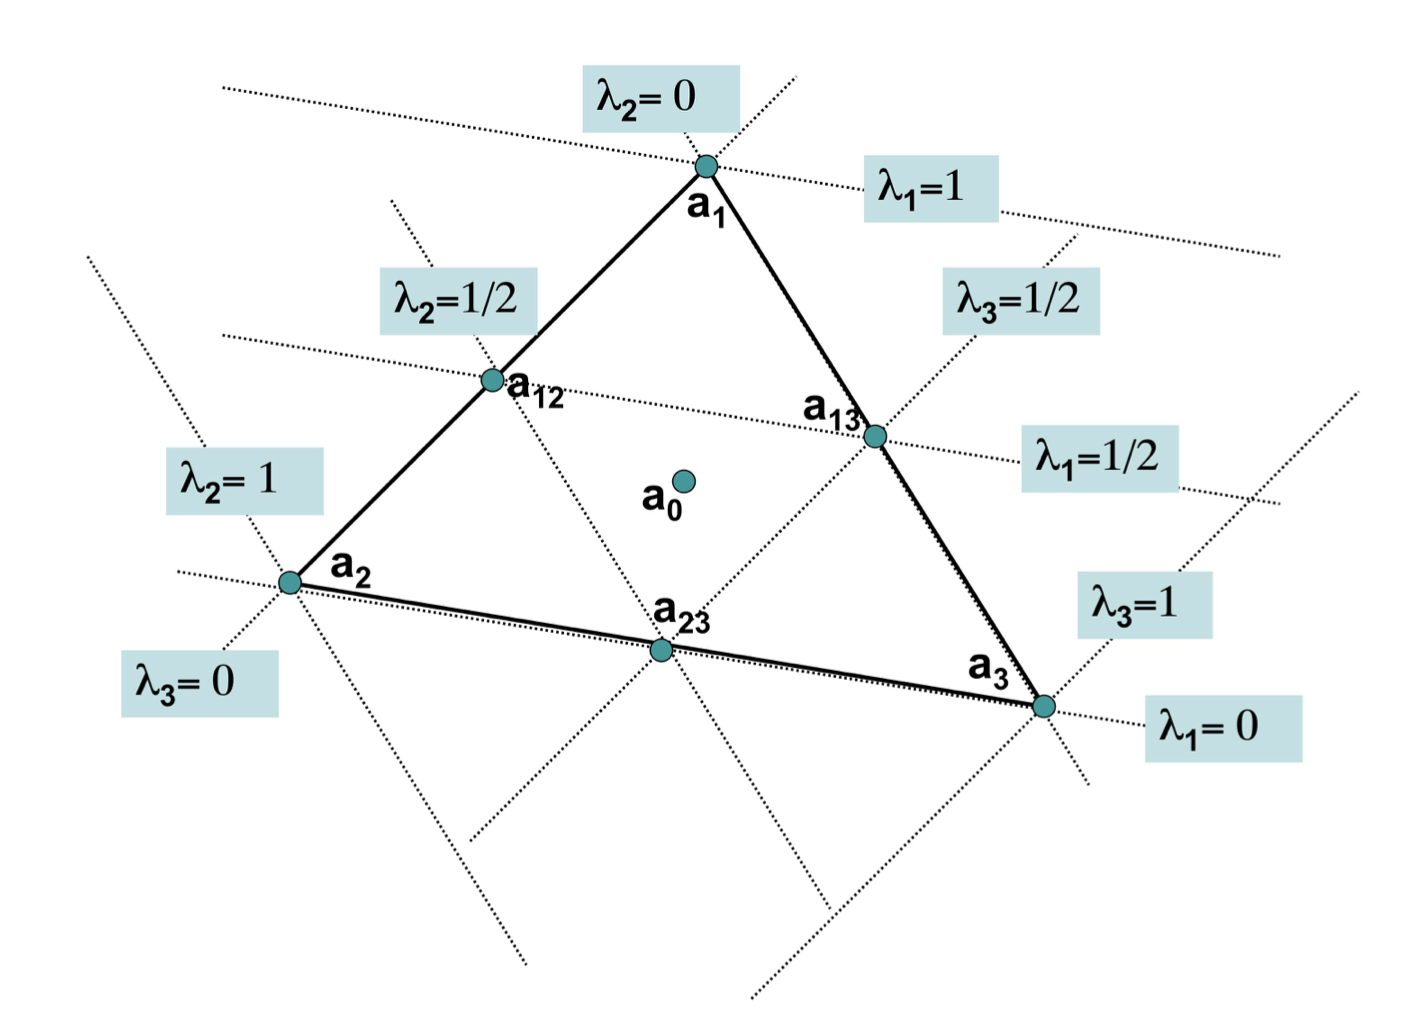
\includegraphics[scale=0.25]{equationsBarycentriques.png} 
\end{center}
\begin{center}
 \begin{tikzpicture}[scale=0.25]
  \draw (10,0)--++(4,1)--++(-1,4)--++(-3,-5);
  \path[fill=orange] (10,0) circle (1.8mm);
   \path[fill=orange] (14,1) circle (1.8mm);
   \path[fill=orange] (13,5) circle (1.8mm);
   
    \path[fill=orange] (10+2,0.5) circle (1.8mm);
   \path[fill=orange] (10+3.5,3) circle (1.8mm);
   \path[fill=orange] (10+1.5,2.5) circle (1.8mm);
\end{tikzpicture}
 \end{center}
\end{frame}
%%%%%%%%%%%%%%%%%%%%%%%%%%%%%%%%%%%%%%%%%%%%%%%%%%%

%%%%%%%%%%%%%%%%%%%%%%%%%%%%%%%%%%%%%%%%%%%%%%%%%%%

\begin{frame}
\frametitle{Éléments finis triangles de type (2)}

\[\begin{array}{l}
\varphi_1(\xi,\eta)=\xi(2\xi-1)\\
\varphi_2(\xi,\eta)=\eta(2\eta-1)\\
\varphi_3(\xi,\eta)=(1-\xi-\eta)(1-2\xi-2\eta)\\
\varphi_{12}(\xi,\eta)=4\xi\eta\\
\varphi_{13}(\xi,\eta)=4\xi(1-\xi-\eta)\\
\varphi_{23}(\xi,\eta)=4\eta(1-\xi-\eta)\\
\end{array}\]

\begin{center}
 \begin{tikzpicture}[scale=0.5]   
   
\draw [domain=0:8] plot(\x,3/32*\x*\x-11/8*\x+3);
\draw [domain=0:6] plot(\x,1/24*\x*\x-1/4*\x+3);
\draw [domain=6:12,gray!80] plot(\x,1/24*\x*\x-1/4*\x+3);
\fill[color=gray!20]
 plot [domain=0:4](\x,3/32*\x*\x-11/8*\x+3)
-- (6,3) 
-- plot [domain=6:0](\x,1/24*\x*\x-1/4*\x+3);
\fill[color=gray!20]
 plot [domain=4:8](\x,3/32*\x*\x-11/8*\x+3);
 -- (4,-1);
 \fill[color=gray!3]
 plot [domain=6:12](\x,1/24*\x*\x-1/4*\x+3)
 -- (12,6)--(8,-2)--(4,-1)--cycle;
 \draw[olive,dashed,->] (0,0)--(0,3);
 \draw (0,0)--(8,-2)--(12,6)--cycle;
 \path[fill=orange] (0,0) circle (1.8mm);
   \path[fill=orange] (8,-2) circle (1.8mm);
   \path[fill=orange] (12,6) circle (1.8mm);
   \path[fill=orange] (4,-1) circle (1.8mm);
   \path[fill=orange] (6,3) circle (1.8mm);
   \path[fill=orange] (10,2) circle (1.8mm);
\end{tikzpicture}
 \end{center}

%\begin{center}
% \begin{tikzpicture}[scale=1.5]   
%\fill[color=gray!20]
%(1,0) -- (1,1)
%-- plot [domain=1:2] (\x,1/\x)
%-- (2,0) -- cycle;
%\end{tikzpicture}
% \end{center}
 
\end{frame}
%%%%%%%%%%%%%%%%%%%%%%%%%%%%%%%%%%%%%%%%%%%%%%%%%%%

\begin{frame}
\frametitle{Éléments finis triangles de type (3)}
\begin{itemize}


\item  Pour $k=3$, le triangle de type (3) est obtenu pour
 \[\mathbb{P}=\mathbb{P}_3^2,\quad \Sigma=\Sigma_3^2 = \{a_1,a_2,a_3\}\cup \{a_{112},a_{113},a_{221},a_{223},a_{331},a_{332}\}\cup \{a_{0}\}\]
Les fonctions de base sont les fonctions
\[\varphi_i=\frac 12\lambda_i(3\lambda_i-1)(3\lambda_i-2), \quad 1\leq  i  \leq 3,\] 
\[\varphi_{iij}=\frac 94\lambda_i\lambda_j(3\lambda_i-1) \quad 1\leq  i,j  \leq 3, i\neq j\]
et
  \[\varphi_0 = 27\lambda_1\lambda_2\lambda_3\]
\end{itemize}
\begin{center}
 \begin{tikzpicture}[scale=0.25]   
   \draw (15,0)--++(4,1)--++(-1,4)--++(-3,-5);
   \path[fill=orange] (15,0) circle (1.8mm);
   \path[fill=orange] (19,1) circle (1.8mm);
   \path[fill=orange] (18,5) circle (1.8mm);
   \path[fill=orange] (15+1.33,0.33) circle (1.8mm);
   \path[fill=orange] (15+2.66,0.66) circle (1.8mm);
   \path[fill=orange] (15+3.67,2) circle (1.8mm);
   \path[fill=orange] (15+3.33,3.66) circle (1.8mm);
   \path[fill=orange] (15+2,3.33) circle (1.8mm);
   \path[fill=orange] (15+1.,1.66) circle (1.8mm);
 \path[fill=black] (0,0) circle (0.3mm) [fill=gray];
 \path[fill=orange] (15+2.33,2) circle (1.8mm);
\end{tikzpicture}
 \end{center}

\end{frame}
%%%%%%%%%%%%%%%%%%%%%%%%%%%%%%%%%%%%%%%%%%%%%%%%%%%
\begin{frame}
\frametitle{Éléments finis tétraèdre ($n=3$)}
$K$ est le tétraèdre de sommets $a_1$, $a_2$, $a_3$ et $a_4$. On pose
\begin{itemize}
\item Pour $k=0$, le tétraèdre de type (0) correspond à
\[ \mathbb{P} = \mathbb{P}_0^3=\mathbb{R}=vect(\varphi=1), \quad \Sigma=\Sigma_0^3 = \{a_0\}\]
\item  Pour $k = 1$, le tétraèdre de type (1) est obtenu pour
\[\mathbb{P}=\mathbb{P}_1^3=\mathbb{R}_1[X,Y]=vect(\varphi_i=\lambda_i,1\leq i\leq 4),\quad \Sigma=\Sigma_1^3 = \{a_i\}_{1\leq i\leq 4}\]
\item   Pour $k=2$, le tétraèdre de type (2) est obtenu pour
\[\begin{array}{l  cl}
\mathbb{P}=\mathbb{P}_2^{(3)}&=&vect(1,\xi,\eta,\nu,\xi^2,\eta^2,\nu^2,\xi\eta,\xi\nu,\eta\nu)\\
&=&vect(\varphi_i=\lambda_i(2\lambda_i-1),\; \varphi_{ij}=4\lambda_i\lambda_j)\\
\Sigma=\Sigma_2 &=& \{a_i\}_{1\leq i\leq 4}\cup \{a_{ij}\}_{1\leq i<j\leq 4}
\end{array}
\]
\end{itemize}
Les expressions des fonctions de base relatives à ces exemples de tétraèdre de type (k) sont formellement identiques à celles donnant les fonctions de base de triangle de type (k) .

\end{frame}
%%%%%%%%%%%%%%%%%%%%%%%%%%%%%%%%%%%%%%%%%%%%%%%%%%%

\begin{frame}
\frametitle{Éléments finis parallélotopes}
\begin{center}
 \begin{tikzpicture}[scale=0.2]
  \draw (0,0)--++(6,0)--++(0,6)--++(-6,0)--++(0,-6);
  \path[fill=red] (3,3) circle (1.8mm);
  \draw (8,0)--++(6,0)--++(0,6)--++(-6,0)--++(0,-6);
  \path[fill=red] (8+0,0) circle (1.8mm);
  \path[fill=red] (8+6,0) circle (1.8mm);
  \path[fill=red] (8+6,6) circle (1.8mm);
  \path[fill=red] (8+0,6) circle (1.8mm);
  \draw (16,0)--++(6,0)--++(0,6)--++(-6,0)--++(0,-6);
  \path[fill=red] (16+0,0) circle (1.8mm);
  \path[fill=red] (16+6,0) circle (1.8mm);
  \path[fill=red] (16+6,6) circle (1.8mm);
  \path[fill=red] (16+0,6) circle (1.8mm);
  \path[fill=red] (16+3,3) circle (1.8mm);
  
  \path[fill=red] (16+0,3) circle (1.8mm);
  \path[fill=red] (16+3,0) circle (1.8mm);
  \path[fill=red] (16+3,6) circle (1.8mm);
  \path[fill=red] (16+6,3) circle (1.8mm);
  
  \draw (24,0)--++(6,0)--++(0,6)--++(-6,0)--++(0,-6);
  \path[fill=red] (24+0,0) circle (1.8mm);
  \path[fill=red] (24+6,0) circle (1.8mm);
  \path[fill=red] (24+6,6) circle (1.8mm);
  \path[fill=red] (24+0,6) circle (1.8mm);
  \path[fill=red] (24+2,0) circle (1.8mm);
  \path[fill=red] (24+2,6) circle (1.8mm);
  \path[fill=red] (24+4,0) circle (1.8mm);
  \path[fill=red] (24+4,6) circle (1.8mm);
  \path[fill=red] (24+0,2) circle (1.8mm);
  \path[fill=red] (24+6,2) circle (1.8mm);
  \path[fill=red] (24+0,4) circle (1.8mm);
  \path[fill=red] (24+6,4) circle (1.8mm);
  
  \path[fill=red] (24+2,2) circle (1.8mm);
  \path[fill=red] (24+4,2) circle (1.8mm);
  \path[fill=red] (24+2,4) circle (1.8mm);
  \path[fill=red] (24+4,4) circle (1.8mm);
  
  
  \draw (34,0)--++(6,0)--++(0,6)--++(-6,0)--++(0,-6);
  \path[fill=black!30!red] (34+0,0) circle (1.8mm);
  \path[fill=black!30!red] (34+6,0) circle (1.8mm);
  \path[fill=black!30!red] (34+6,6) circle (1.8mm);
  \path[fill=black!30!red] (34+0,6) circle (1.8mm);
  
  \path[fill=black!30!red] (34+3,0) circle (1.8mm);
  \path[fill=black!30!red] (34+3,6) circle (1.8mm);
  \path[fill=black!30!red] (34,3) circle (1.8mm);
  \path[fill=black!30!red] (34+6,3) circle (1.8mm);
  
  \draw (42,0)--++(6,0)--++(0,6)--++(-6,0)--++(0,-6);
  \path[fill=black!30!red] (42+0,0) circle (1.8mm);
  \path[fill=black!30!red] (42+6,0) circle (1.8mm);
  \path[fill=black!30!red] (42+6,6) circle (1.8mm);
  \path[fill=black!30!red] (42+0,6) circle (1.8mm);
  \path[fill=black!30!red] (42+2,0) circle (1.8mm);
  \path[fill=black!30!red] (42+2,6) circle (1.8mm);
  \path[fill=black!30!red] (42+4,0) circle (1.8mm);
  \path[fill=black!30!red] (42+4,6) circle (1.8mm);
  \path[fill=black!30!red] (42+0,2) circle (1.8mm);
  \path[fill=black!30!red] (42+6,2) circle (1.8mm);
  \path[fill=black!30!red] (42+0,4) circle (1.8mm);
  \path[fill=black!30!red] (42+6,4) circle (1.8mm);
  
  
  
   \end{tikzpicture}
 \end{center}
 
 %%%%%%%%%%%%%%%%%%%%%%%%%%%%%%%%%%%%%%%%%%%%%%%%%%
 
 \begin{center}
 \begin{tikzpicture}[scale=0.25]
  \draw (0,0)--++(4,0)--++(2.2,2.2)--++(0,4)--++(-4,0)--++(-2.2,-2.2)--++(4,0)--++(0,-4);
  \draw (0,0)--++(0,4)--++(4,0)--++(2.2,2.2);
  \draw[dotted,->] (2.2,2.2)--++(-3.3,-3.3);
  \draw[dotted,->] (2.2,2.2)--++(5.3,0);
  \draw[dotted,->] (2.2,2.2)--++(0,5.3);
   \path[fill=black!60!green] (0,0) circle (1.8mm);  
  \path[fill=black!60!green] (4,0) circle (1.8mm);
  \path[fill=black!60!green] (6.2,2.2) circle (1.8mm);
  \path[fill=black!60!green] (2.2,2.2) circle (1.8mm);
  
  \path[fill=black!60!green] (0,4) circle (1.8mm);  
  \path[fill=black!60!green] (4,4) circle (1.8mm);
  \path[fill=black!60!green] (6.2,6.2) circle (1.8mm);
  \path[fill=black!60!green] (2.2,6.2) circle (1.8mm);
  
  \draw (10,0)--++(4,0)--++(2.2,2.2)--++(0,4)--++(-4,0)--++(-2.2,-2.2)--++(4,0)--++(0,-4);
  \draw (10,0)--++(0,4)--++(4,0)--++(2.2,2.2);
  \draw[dotted,->] (10+2.2,2.2)--++(-3.3,-3.3);
  \draw[dotted,->] (10+2.2,2.2)--++(5.3,0);
  \draw[dotted,->] (10+2.2,2.2)--++(0,5.3);
  
  \path[fill=black!60!green] (10+0,0) circle (1.8mm);  
  \path[fill=black!60!green] (10+4,0) circle (1.8mm);
  \path[fill=black!60!green] (10+6.2,2.2) circle (1.8mm);
  \path[fill=black!60!green] (10+2.2,2.2) circle (1.8mm);
  
  \path[fill=black!60!green] (10+0,4) circle (1.8mm);  
  \path[fill=black!60!green] (10+4,4) circle (1.8mm);
  \path[fill=black!60!green] (10+6.2,6.2) circle (1.8mm);
  \path[fill=black!60!green] (10+2.2,6.2) circle (1.8mm);
  
  \path[fill=black!60!green] (10+2,0) circle (1.8mm);  
  \path[fill=black!60!green] (10+4+1.1,0+1.1) circle (1.8mm);
  \path[fill=black!60!green] (10+4.2,2.2) circle (1.8mm);
  \path[fill=black!60!green] (10+1.1,1.1) circle (1.8mm);
  
  \path[fill=black!60!green] (10+2,4) circle (1.8mm);  
  \path[fill=black!60!green] (10+4+1.1,0+1.1+4) circle (1.8mm);
  \path[fill=black!60!green] (10+4.2,2.2+4) circle (1.8mm);
  \path[fill=black!60!green] (10+1.1,1.1+4) circle (1.8mm);
  
  \path[fill=black!60!green] (10+0,2) circle (1.8mm); 
  \path[fill=black!60!red] (10+2,2) circle (1.8mm); 
  \path[fill=black!60!green] (10+4,2) circle (1.8mm);
  \path[fill=black!60!green] (10+6.2,4.2) circle (1.8mm);
  \path[fill=black!60!red] (10+5.1,4.2) circle (1.8mm);% ici ici
  \path[fill=black!60!green] (10+2.2,4.2) circle (1.8mm);
  
    \draw (20,0)--++(6.2,2.2)--++(0,4)--++(-6.2,-2.2)--++(0,-4);
    \draw (20+2.2,6.2)--++(-2.3,-2.3);
  \draw (20+2.2,6.2)--++(4,0);
  %\draw (0,0)--++(0,4)--++(4,0)--++(2.2,2.2);
  \draw[dotted,->] (20+2.2,2.2)--++(-3.3,-3.3);
  \draw[dotted,->] (20+2.2,2.2)--++(5.3,0);
  \draw[dotted,->] (20+2.2,2.2)--++(0,5.3);
   \path[fill=black!60!green] (20,0) circle (1.8mm);  
  %\path[fill=black!60!green] (4,0) circle (1.8mm);
  \path[fill=black!60!green] (20+6.2,2.2) circle (1.8mm);
  \path[fill=black!60!green] (20+2.2,2.2) circle (1.8mm);
  
  \path[fill=black!60!green] (20,4) circle (1.8mm);  
  %\path[fill=black!60!green] (4,4) circle (1.8mm);
  \path[fill=black!60!green] (20+6.2,6.2) circle (1.8mm);
  \path[fill=black!60!green] (20+2.2,6.2) circle (1.8mm);
  
      \draw (30,0)--++(6.2,2.2)--++(0,4)--++(-6.2,-2.2)--++(0,-4);
    \draw (30+2.2,6.2)--++(-2.3,-2.3);
  \draw (30+2.2,6.2)--++(4,0);
  %\draw (0,0)--++(0,4)--++(4,0)--++(2.2,2.2);
  \draw[dotted,->] (30+2.2,2.2)--++(-3.3,-3.3);
  \draw[dotted,->] (30+2.2,2.2)--++(5.3,0);
  \draw[dotted,->] (30+2.2,2.2)--++(0,5.3);
  
   \path[fill=black!60!green] (30,0) circle (1.8mm);  
  \path[fill=black!60!green] (30+6.2,2.2) circle (1.8mm);
  \path[fill=black!60!green] (30+2.2,2.2) circle (1.8mm);
  
  \path[fill=black!60!green] (30,4) circle (1.8mm);  
  %\path[fill=black!60!green] (4,4) circle (1.8mm);
  \path[fill=black!60!green] (30+6.2,6.2) circle (1.8mm);
  \path[fill=black!60!green] (30+2.2,6.2) circle (1.8mm);
  
   \path[fill=black!60!green] (30+3.1,1.1) circle (1.8mm);  
  \path[fill=black!60!green] (30+4.2,2.2) circle (1.8mm);
  \path[fill=black!60!green] (30+1.1,1.1) circle (1.8mm);
  
  \path[fill=black!60!green] (30+3.1,1.1+4) circle (1.8mm);  
  \path[fill=black!60!green] (30+4.2,2.2+4) circle (1.8mm);
  \path[fill=black!60!green] (30+1.1,1.1+4) circle (1.8mm);
  
  \path[fill=black!60!green] (30,2) circle (1.8mm);  
  \path[fill=black!60!green] (30+6.2,4.2) circle (1.8mm);
  \path[fill=black!60!green] (30+2.2,4.2) circle (1.8mm);
   \end{tikzpicture}
 \end{center}
 
 
L'enveloppe convexe $K$ de $2^n$ points $a_i$, est un n-parallèlotope si et seulement si il existe une application affine inversible $F$ % de $\mathbb{R}^n$ dans $\mathbb{R}^n$
 telle que
\begin{equation}
a_j=F(\hat{a}_j),\quad 1\leq j\leq 2^n,
\end{equation}
où les points $\hat{a}_j$,  $1\leq j\leq 2^n$,  sont les sommets de $\widehat{K}$, hypercube unité $[0, 1]^n$ de $\mathbb{R}^n$ ;
\begin{itemize}
\item pour $n=2$, $K$ est un parallélogramme.
\item pour $n=3$, $K$ est un parallélépipède.
\end{itemize}


\end{frame}
%%%%%%%%%%%%%%%%%%%%%%%%%%%%%%%%%%%%%%%%%%%%%%%%%%%
\begin{frame}
\frametitle{Éléments finis parallélotopes}
Soit $\mathbb{Q}_k^{(n)}$ l'espace des (fonctions) polynômes de degré inférieur ou égal à $k$ par rapport à chaque variable: 
\begin{equation}
\forall x\in \mathbb{R}^n,\quad p(x)=\sum_{0\leq i_1\leq k,...,0\leq i_n\leq k}\alpha_{i_1,...,i_n}x_1^{\alpha_1}...x_n^{\alpha_n}
\end{equation}
\[\dim (\mathbb{Q}_k) = (k+ 1)^n\]


\begin{itemize}
\item $\mathbb{Q}_0^{(n)}=\mathbb{R}$.
\item $\mathbb{Q}_k^{(1)}=\mathbb{P}_k^{(1)}$.
\item $\mathbb{Q}_k^{(2)}=vect\{x^iy^j;\; 0\leq i,j \leq k\}$, $\dim \mathbb{Q}_k^{(2)}=(k+1)^2$.
En particulier: 
\begin{itemize}
\item $\mathbb{Q}_1^{(2)}=\{a+bx+cy+dxy;\; a,b,c,d\in \mathbb{R}\}$, $\dim \mathbb{Q}_1^{(2)}=4$.
\item $\mathbb{Q}_2^{(2)}=vect\{1,x,x^2,y,y^2,xy,xy^2,x^2y,x^2y^2\}$, $\dim \mathbb{Q}_2^{(2)}=9$.
\end{itemize}
\item $\mathbb{Q}_k^{(3)}=vect\{x^py^qz^r;\; 0\leq p,q,r \leq k\}$, $\dim \mathbb{Q}_k^{(2)}=(k+1)^3$.
Et donc: 
\begin{itemize}
\item $\mathbb{Q}_1^{(3)}=vect\{1,x,y,z,xy,xz,yz,xyz\}$, $\dim \mathbb{Q}_1^{(2)}=8$.
\item $\mathbb{Q}_1^{(3)}=vect\left\{
1,x,x^2,y,y^2,z,z^2,xy,xz,yz,xyz,x^2y,x^2z,x^2yz,xy^2,\right.$
$\left. ,y^2z,xy^2z,xz^2,yz^2,xyz^2,x^2y^2,x^2z^2,y^2z^2,x^2y^2z,x^2yz^2,xy^2z^2,x^2y^2z^2\right\}$
$\dim \mathbb{Q}_1^{(2)}=27$.
\end{itemize}
\end{itemize}

   On prend alors pour domaine $\widehat{K}$ l'hypercube unité $[0, 1]^n$ de $\mathbb{R}^n$ et on définit pour tout entier $k \geq 1$ l'ensemble de points de $\widehat{K}$
\begin{equation}
\widehat{\Xi}_k^{(n)}=\left\{\hat{x}=(\hat{x}_i)_{1\leq i\leq n};\, \hat{x}_i\in\left\{0,\frac 1k,...,\frac{k-1}{k},1\right\},\; 1\leq i\leq n\right\}
\end{equation}
\end{frame}
%%%%%%%%%%%%%%%%%%%%%%%%%%%%%%%%%%%%%%%%%%%%%%%%%%%
%%%%%%%%%%%%%%%%%%%%%%%%%%%%%%%%%%%%%%%%%%%%%%%%%%%
\begin{frame}
\frametitle{Éléments finis parallélotopes}


   On prend alors pour domaine $\widehat{K}$ l'hypercube unité $[0, 1]^n$ de $\mathbb{R}^n$ et on définit pour tout entier $k \geq 1$ l'ensemble de points de $\widehat{K}$
\begin{equation}
\widehat{\Xi}_k^{(n)}=\left\{\hat{x}=(\hat{x}_i)_{1\leq i\leq n};\, \hat{x}_i\in\left\{0,\frac 1k,...,\frac{k-1}{k},1\right\},\; 1\leq i\leq n\right\}
\end{equation}
Pour $k=0$, on posera  
\begin{equation}
\widehat{\Xi}_0^{(n)}=\left\{\left(\frac 1{n+1},...,\frac 1{n+1}\right)\in \mathbb{R}^n \right\}
\end{equation}
On a ainsi pour tout entier  $k\geq 1$                                                                                            \[\mbox{card} (\widehat{\Xi}_k) =  (k+ 1)^n\]
\end{frame}
%%%%%%%%%%%%%%%%%%%%%%%%%%%%%%%%%%%%%%%%%%%%%%%%%%%
%%%%%%%%%%%%%%%%%%%%%%%%%%%%%%%%%%%%%%%%%%%%%%%%%%%
\begin{frame}
\frametitle{Éléments finis parallélotopes en dimension 1}
 $\widehat{K}$ est le segment $[0, 1]$ 
\[
\widehat{\Xi}_0^{(1)}=\left\{\frac 1{2}\right\},\quad \mbox{pour }k \geq 1, \; \widehat{\Xi}_k^{(1)}=\left\{0,\frac 1k,...,\frac{k-1}{k},1\right\}
\]
 \[\mbox{card} (\widehat{\Xi}_k) =  k+ 1\] En particulier
 \begin{itemize}
\item $\widehat{\Xi}_1^{(1)}=\left\{0,1\right\}$, Card$\widehat{\Xi}_1^{(1)}=2$
\item $\widehat{\Xi}_2^{(1)}=\left\{0,\frac 12,1\right\}$, Card$\widehat{\Xi}_2^{(1)}=3$
\item $\widehat{\Xi}_3^{(1)}=\left\{0,\frac 13,\frac 23,1\right\}$, Card$\widehat{\Xi}_3^{(1)}=4$
 \end{itemize}
\end{frame}
%%%%%%%%%%%%%%%%%%%%%%%%%%%%%%%%%%%%%%%%%%%%%%%%%%%
%%%%%%%%%%%%%%%%%%%%%%%%%%%%%%%%%%%%%%%%%%%%%%%%%%%
\begin{frame}
\frametitle{Éléments finis parallélotopes en dimension 2}
 $\widehat{K}$ est le carré $[0, 1]^2$. On pose $\hat{a}_1=(0,0)$, $\hat{a}_2=(1,0)$, $\hat{a}_3=(1,1)$, $\hat{a}_4=(0,1)$, 
\[
\widehat{\Xi}_0^{(2)}=\left\{(\frac 1{2},\frac 1{2})\right\},\; \mbox{pour }k \geq 1, \; \widehat{\Xi}_k^{(2)}=\left\{(\hat{x}_1,\hat{x}_2);\; \hat{x}_i \in\left\{0,\frac 1k,...,\frac{k-1}{k},1\right\}\right\}
\]
 \[\mbox{card} (\widehat{\Xi}_k) =  (k+ 1)^2\] 
 \begin{itemize}
\item $\widehat{\Xi}_1^{(2)}=\left\{(\hat{x}_1,\hat{x}_2);\; \hat{x}_i \in\left\{0,1\right\}\right\}=\left\{\hat{a}_1,\hat{a}_2,\hat{a}_3,\hat{a}_4\right\}$, Card$\widehat{\Xi}_2^{(1)}=4$
\item $\widehat{\Xi}_2^{(1)}=\left\{(\hat{x}_1,\hat{x}_2);\; \hat{x}_i \in\left\{0,\frac 12,1\right\}\right\}=\left\{\hat{a}_0,\hat{a}_1,\hat{a}_2,\hat{a}_3,\hat{a}_4,\hat{a}_{12},\hat{a}_{13},\hat{a}_{14},\hat{a}_{23},\hat{a}_{24},\hat{a}_{34}\right\}$, Card$\widehat{\Xi}_2^{(1)}=9$
\item $\widehat{\Xi}_3^{(2)}=\left\{(\hat{x}_1,\hat{x}_2);\; \hat{x}_i \in\left\{0,\frac 13,\frac 23,1\right\}\right\}$, Card$\widehat{\Xi}_3^{(2)}=16$
 \end{itemize}
 \begin{center}
 \begin{tikzpicture}[scale=0.2]
  \draw (0,0)--++(6,0)--++(0,6)--++(-6,0)--++(0,-6);
  \path[fill=red] (3,3) circle (1.8mm);
  \draw (8,0)--++(6,0)--++(0,6)--++(-6,0)--++(0,-6);
  \path[fill=red] (8+0,0) circle (1.8mm);
  \path[fill=red] (8+6,0) circle (1.8mm);
  \path[fill=red] (8+6,6) circle (1.8mm);
  \path[fill=red] (8+0,6) circle (1.8mm);
  \draw (16,0)--++(6,0)--++(0,6)--++(-6,0)--++(0,-6);
  \path[fill=red] (16+0,0) circle (1.8mm);
  \path[fill=red] (16+6,0) circle (1.8mm);
  \path[fill=red] (16+6,6) circle (1.8mm);
  \path[fill=red] (16+0,6) circle (1.8mm);
  \path[fill=red] (16+3,3) circle (1.8mm);
  
  \path[fill=red] (16+0,3) circle (1.8mm);
  \path[fill=red] (16+3,0) circle (1.8mm);
  \path[fill=red] (16+3,6) circle (1.8mm);
  \path[fill=red] (16+6,3) circle (1.8mm);
  
  \draw (24,0)--++(6,0)--++(0,6)--++(-6,0)--++(0,-6);
  \path[fill=red] (24+0,0) circle (1.8mm);
  \path[fill=red] (24+6,0) circle (1.8mm);
  \path[fill=red] (24+6,6) circle (1.8mm);
  \path[fill=red] (24+0,6) circle (1.8mm);
  \path[fill=red] (24+2,0) circle (1.8mm);
  \path[fill=red] (24+2,6) circle (1.8mm);
  \path[fill=red] (24+4,0) circle (1.8mm);
  \path[fill=red] (24+4,6) circle (1.8mm);
  \path[fill=red] (24+0,2) circle (1.8mm);
  \path[fill=red] (24+6,2) circle (1.8mm);
  \path[fill=red] (24+0,4) circle (1.8mm);
  \path[fill=red] (24+6,4) circle (1.8mm);
  
  \path[fill=red] (24+2,2) circle (1.8mm);
  \path[fill=red] (24+4,2) circle (1.8mm);
  \path[fill=red] (24+2,4) circle (1.8mm);
  \path[fill=red] (24+4,4) circle (1.8mm);

 \end{tikzpicture}
   \end{center}
\end{frame}
%%%%%%%%%%%%%%%%%%%%%%%%%%%%%%%%%%%%%%%%%%%%%%%%%%%
%%%%%%%%%%%%%%%%%%%%%%%%%%%%%%%%%%%%%%%%%%%%%%%%%%%
\begin{frame}
\frametitle{Éléments finis parallélotopes en dimension 3}
 $\widehat{K}$ est le cube $[0, 1]^3$. On pose $\hat{a}_1=(0,0,0)$, $\hat{a}_2=(1,0,0)$, $\hat{a}_3=(1,1,0)$, $\hat{a}_4=(0,1,0)$, $\hat{a}_5=(0,0,1)$, $\hat{a}_6=(1,0,1)$, $\hat{a}_7=(1,1,1)$, $\hat{a}_8=(0,1,1)$, 
\[
\widehat{\Xi}_0^{(3)}=\left\{(\frac 1{2},\frac 1{2},\frac 1{2})\right\},\; \; \widehat{\Xi}_k^{(3)}=\left\{(\hat{x}_1,\hat{x}_2,\hat{x}_3);\; \hat{x}_i \in\left\{0,\frac 1k,...,\frac{k-1}{k},1\right\}\right\}
\]
 \[\mbox{card} (\widehat{\Xi}_k) =  (k+ 1)^3\] 
 \begin{itemize}
\item $\widehat{\Xi}_1^{(3)}=\left\{(\hat{x}_1,\hat{x}_2,\hat{x}_3);\; \hat{x}_i \in\left\{0,1\right\}\right\}=\left\{\hat{a}_1,\hat{a}_2,\hat{a}_3,\hat{a}_4,\hat{a}_5,\hat{a}_6,\hat{a}_7,\hat{a}_8\right\}$, Card$=8$
\item $\widehat{\Xi}_2^{(3)}=\left\{(\hat{x}_1,\hat{x}_2,\hat{x}_3));\; \hat{x}_i \in\left\{0,\frac 12,1\right\}\right\}$, Card$\widehat{\Xi}_2^{(3)}=27$
 \end{itemize}
 \begin{center}
 \begin{tikzpicture}[scale=0.2]
  \draw (0,0)--++(6,0)--++(0,6)--++(-6,0)--++(0,-6);
  \path[fill=red] (3,3) circle (1.8mm);
  \draw (8,0)--++(6,0)--++(0,6)--++(-6,0)--++(0,-6);
  \path[fill=red] (8+0,0) circle (1.8mm);
  \path[fill=red] (8+6,0) circle (1.8mm);
  \path[fill=red] (8+6,6) circle (1.8mm);
  \path[fill=red] (8+0,6) circle (1.8mm);
  \draw (16,0)--++(6,0)--++(0,6)--++(-6,0)--++(0,-6);
  \path[fill=red] (16+0,0) circle (1.8mm);
  \path[fill=red] (16+6,0) circle (1.8mm);
  \path[fill=red] (16+6,6) circle (1.8mm);
  \path[fill=red] (16+0,6) circle (1.8mm);
  \path[fill=red] (16+3,3) circle (1.8mm);
  
  \path[fill=red] (16+0,3) circle (1.8mm);
  \path[fill=red] (16+3,0) circle (1.8mm);
  \path[fill=red] (16+3,6) circle (1.8mm);
  \path[fill=red] (16+6,3) circle (1.8mm);
  
  \draw (24,0)--++(6,0)--++(0,6)--++(-6,0)--++(0,-6);
  \path[fill=red] (24+0,0) circle (1.8mm);
  \path[fill=red] (24+6,0) circle (1.8mm);
  \path[fill=red] (24+6,6) circle (1.8mm);
  \path[fill=red] (24+0,6) circle (1.8mm);
  \path[fill=red] (24+2,0) circle (1.8mm);
  \path[fill=red] (24+2,6) circle (1.8mm);
  \path[fill=red] (24+4,0) circle (1.8mm);
  \path[fill=red] (24+4,6) circle (1.8mm);
  \path[fill=red] (24+0,2) circle (1.8mm);
  \path[fill=red] (24+6,2) circle (1.8mm);
  \path[fill=red] (24+0,4) circle (1.8mm);
  \path[fill=red] (24+6,4) circle (1.8mm);
  
  \path[fill=red] (24+2,2) circle (1.8mm);
  \path[fill=red] (24+4,2) circle (1.8mm);
  \path[fill=red] (24+2,4) circle (1.8mm);
  \path[fill=red] (24+4,4) circle (1.8mm);

 \end{tikzpicture}
   \end{center}
\end{frame}
%%%%%%%%%%%%%%%%%%%%%%%%%%%%%%%%%%%%%%%%%%%%%%%%%%%
\begin{frame}
\frametitle{Éléments finis parallélotopes}

\begin{itemize}
\item Théorème: Pour tout entier $k\geq 0$, l'ensemble $\widehat{\Xi}_k$ est $\mathbb{Q}_k$-unisolvant.
\item Définition: On appelle $n-$hypercube unité de type ($k$),  l'élément fini $(K, \mathbb{Q}_k, \widehat{\Xi}_k)$. On appelle $n-$parallèlotope de type ($k$) tout élément fini $(K, P, \Sigma)$ affine-équivalent au $n-$hypercube unité de. type ($k$).
\item le $n-$hypercube unité de type ($k$) est un carré unité de type ($k$) lorsque $n=2$, 
\item et cube unité de type ($k$) lorsque $n = 3$
\end{itemize}
\end{frame}
%%%%%%%%%%%%%%%%%%%%%%%%%%%%%%%%%%%%%%%%%%%%%%%%%%%
\begin{frame}
\frametitle{Éléments finis parallélotopes}
Dire que $(K, P, \Sigma)$ est un $n$-parallèlotope de type 
($k$) signifie donc qu'il existe une application affine inversible $F$ de $\mathbb{R}^n$ sur $\mathbb{R}^n$ telle que
\begin{equation}
K=F(\widehat{K}),\quad \mathbb{P}=\{p: \mathbb{R}^n\to \mathbb{R}^n;\; p\circ F\in \mathbb{Q}_k\},\quad \Sigma=F(\widehat{\Xi}_k).
\end{equation}
Supposons $n=2$ pour simplifier un peu l'exposé :
\begin{enumerate}
\item $K$ est un parallélogramme de $\mathbb{R}^n$;
\item pour $k=0$, $\Sigma$ est le centre du parallélogramme $K$ ; pour $k =1$, $\Sigma$ est l'ensemble des sommets ; pour $k =2$, $\Sigma$ est l'ensemble constitué des sommets de $K$, des milieux des côtés de $K$ et du centre de $K$, etc.
\item l'espace $\mathbb{P}$ est un espace de polynômes tel que
\[\mathbb{P}_k\subset \mathbb{P}\subset \mathbb{P}_{2k}\]
\end{enumerate}

cet espace $\mathbb{P}$ ne coïncide avec l'espace $\mathbb{Q}_k$ que dans le cas particulier où $K$ est un rectangle de côtés parallèles aux axes.
\end{frame}
%%%%%%%%%%%%%%%%%%%%%%%%%%%%%%%%%%%%%%%%%%%%%%%%%%%

\begin{frame}
\frametitle{Éléments finis parallélotopes}
  Dans le cas $n = 2$;  $\widehat{K}$ est le carré unité de $\mathbb{R}^2$. Nous noterons $(\hat{x}_1, \hat{x}_2)$ les coordonnées cartésiennes du point courant $\hat{x}$ de $\widehat{K}$, de sommets

\begin{equation}
\hat{a}_1=(0,0),\quad \hat{a}_2=(1,0),\quad \hat{a}_3=(1,1),\quad \hat{a}_4=(0,1)
\end{equation} 
Il sera commode de poser
\begin{equation}
\hat{x}_3=1-\hat{x}_1,\quad \hat{x}_4=1-\hat{x}_2
\end{equation}
et d'associer à tout entier $i$ l'entier $\bar{i}$ congru à $i$ modulo 4 et compris entre 1 et 4.  En particulier, un sommet $\hat{a}_i$, $1\leq i \leq  4$, est alors défini par les relations
\[\hat{x}_{\bar{i}}=\hat{x}_{\overline{i+1}}=0\]

\end{frame}
%%%%%%%%%%%%%%%%%%%%%%%%%%%%%%%%%%%%%%%%%%%%%%%%%%%

\begin{frame}
\frametitle{Éléments finis parallélotopes}
  Explicitons les fonctions de base de l'élément fini $(\widehat{K},\widehat{\mathbb{P}},\widehat{\Sigma})$ carré unité de type ($k$), pour les premières valeurs de $k$.
\begin{itemize}
\item Pour $k=0$, le carré unité de type (0) est obtenu pour
\[\widehat{\mathbb{P}} = \mathbb{Q}_0, = P_0 ,\quad \widehat{\Sigma} =\widehat{\Xi}_0=\{\hat{a}_0\}\]
où $\hat{a}_0$ est le centre du carré, $\hat{a}_0=\frac 14(\hat{a}_1+\hat{a}_2+\hat{a}_3+\hat{a}_4)$. La fonction de base $\widehat{\varphi}_0$, est la fonction constante égale à 1.
\end{itemize}
\end{frame}
%%%%%%%%%%%%%%%%%%%%%%%%%%%%%%%%%%%%%%%%%%%%%%%%%%%

\begin{frame}
\frametitle{Le carré de type (1) ou (2)}
  \begin{itemize}
\item  Pour $k = 1$, le carré de type (1) correspond à
\[\widehat{\mathbb{P}} = \mathbb{Q}_1,\quad \widehat{\Sigma} =\widehat{\Xi}_1^{(2)}=\{\hat{a}_i\}_{1\leq i\leq 4}\]
Les fonctions de base s'écrivent
\[\widehat{\varphi}_i(\hat{x})=\hat{x}_{\overline{i+2}}\hat{x}_{\overline{i+3}},\quad 1\leq i\leq 4\]

\item  Pour $k=2$, le carré de type (2) est obtenu pour
\[\widehat{\mathbb{P}} = \mathbb{Q}_2, = P_0 ,\quad \widehat{\Sigma} =\widehat{\Xi}_2^{(2)}=\{\hat{a}_i\}_{1\leq i\leq 9}\]
où les points $\hat{a}_i$ , $5\leq i \leq 8$, sont les milieux des côtés $[\hat{a}_i \hat{a}_{i+1}]$ et le point $\hat{a}_9$ est le centre du carré. Les fonctions de base sont

\begin{equation}
  \begin{array}{l}
  \widehat{\varphi}_i(\hat{x})=\hat{x}_{\overline{i+2}}(2\hat{x}_{\overline{i+2}}-1)\hat{x}_{\overline{i+3}}(2\hat{x}_{\overline{i+3}}-1),\quad 1\leq i\leq 4,\\
  \widehat{\varphi}_i(\hat{x})=-4\hat{x}_{\overline{i+2}}(\hat{x}_{\overline{i+2}}-1)\hat{x}_{\overline{i+3}}(2\hat{x}_{\overline{i+3}}-1),\quad 5\leq i\leq 8,\\
  \widehat{\varphi}_9(\hat{x})=16 \hat{x}_1\hat{x}_2\hat{x}_3\hat{x}_4.
\end{array}              
\end{equation}
\end{itemize}
\end{frame}
%%%%%%%%%%%%%%%%%%%%%%%%%%%%%%%%%%%%%%%%%%%%%%%%%%%


\begin{frame}
\frametitle{Éléments finis parallélotopes}
A partir des deux derniers exemples de carré unité, 
on peut construire des éléments fini qui seront de mise en œuvre informatique 
plus simple sans que cela nuise à la précision. l'élément fini $(\widehat{K},\widehat{\mathbb{P}},\widehat{\Sigma})$ obtenu vérifiera
\[\widehat{\Sigma}=\widehat{\Xi}_2\cap \partial \widehat{K}\quad \mbox{ et }\quad\mathbb{P}_2 \subset \widehat{\mathbb{P}} \subset \widehat{\mathbb{Q}}_2\]
 On pose
\begin{equation}
\left\{
\begin{array}{l}
\widehat{\Sigma}=\widehat{\Xi}_2^\star=\{\hat{a}_i\}_{1\leq i\leq 8}\\
\widehat{\mathbb{P}}=\widehat{\mathbb{Q}}_2^\star=\{q(x)+\alpha_1x_1^2x_2+\alpha_2x_1x_2^2,\quad q\in\mathbb{P}_2,\quad (\alpha_1, \alpha_2)\in \mathbb{R}^2\}
\end{array} \right.
\end{equation}
On remarque que l'espace $\mathbb{Q}_2 = \mathbb{Q}_2^\star \oplus vect\{x_1^2x_2^2\}$% est somme directe de $\mathbb{Q}_2^\star$ et de l'espace engendré par le monôme $x_1^2x_2^2$.
\begin{itemize}
\item L'ensemble $\widehat{\Xi}_2^\star$ est $\mathbb{Q}_2^\star$-unisolvant.
\item on vérifie que les fonctions 
\begin{equation}
  \begin{array}{l}
  \hat{\varphi}_i(\hat{x})=\hat{x}_{\overline{i+2}} \hat{x}_{\overline{i+3}}  (2\hat{x}_{\overline{i+2}}+2\hat{x}_{\overline{i+3}}-3),\quad 1\leq i\leq 4,\\
  \hat{\varphi}_i(\hat{x})=-4\hat{x}_{\overline{i+2}}(\hat{x}_{\overline{i+2}}-1)\hat{x}_{\overline{i+3}},\quad 5\leq i\leq 8.
\end{array}              
\end{equation}
sont les fonctions de base de $(\widehat{K},\mathbb{Q}_2^\star,\widehat{\Sigma}_2^\star)$.
\end{itemize}
\end{frame}
%%%%%%%%%%%%%%%%%%%%%%%%%%%%%%%%%%%%%%%%%%%%%%%%%%%


\begin{frame}
\frametitle{Éléments finis parallélotopes}

En dimension $n = 3$, on vous laisse le soin de décrire en détail l'élément 
fini $(\widehat{K},\widehat{\mathbb{P}},\widehat{\Sigma})$  cube unité de type ($k$), pour les valeurs $k=0, 1, 2$. Par exemple, 
pour $k = 1$, l'ensemble $\widehat{\Sigma}$ est constitué par les 8 sommets du cube.

  Pour $k=2$, on préfère utiliser le cube unité de type (2)* où l'ensemble $\Sigma$ 
est constitué par les 8 sommets du cube et les milieux des 12 arêtes de ce cube.

\begin{center}
 \begin{tikzpicture}[scale=0.45]
  \draw (0,0)--++(4,0)--++(2.2,2.2)--++(0,4)--++(-4,0)--++(-2.2,-2.2)--++(4,0)--++(0,-4);
  \draw (0,0)--++(0,4)--++(4,0)--++(2.2,2.2);
  \draw[dotted,->] (2.2,2.2)--++(-3.3,-3.3);
  \draw[dotted,->] (2.2,2.2)--++(5.3,0);
  \draw[dotted,->] (2.2,2.2)--++(0,5.3);
   \path[fill=black!60!green] (0,0) circle (1.8mm);  
  \path[fill=black!60!green] (4,0) circle (1.8mm);
  \path[fill=black!60!green] (6.2,2.2) circle (1.8mm);
  \path[fill=black!60!green] (2.2,2.2) circle (1.8mm);
  
  \path[fill=black!60!green] (0,4) circle (1.8mm);  
  \path[fill=black!60!green] (4,4) circle (1.8mm);
  \path[fill=black!60!green] (6.2,6.2) circle (1.8mm);
  \path[fill=black!60!green] (2.2,6.2) circle (1.8mm);
  
  \draw (10,0)--++(4,0)--++(2.2,2.2)--++(0,4)--++(-4,0)--++(-2.2,-2.2)--++(4,0)--++(0,-4);
  \draw (10,0)--++(0,4)--++(4,0)--++(2.2,2.2);
  \draw[dotted,->] (10+2.2,2.2)--++(-3.3,-3.3);
  \draw[dotted,->] (10+2.2,2.2)--++(5.3,0);
  \draw[dotted,->] (10+2.2,2.2)--++(0,5.3);
  
  \path[fill=black!60!green] (10+0,0) circle (1.8mm);  
  \path[fill=black!60!green] (10+4,0) circle (1.8mm);
  \path[fill=black!60!green] (10+6.2,2.2) circle (1.8mm);
  \path[fill=black!60!green] (10+2.2,2.2) circle (1.8mm);
  
  \path[fill=black!60!green] (10+0,4) circle (1.8mm);  
  \path[fill=black!60!green] (10+4,4) circle (1.8mm);
  \path[fill=black!60!green] (10+6.2,6.2) circle (1.8mm);
  \path[fill=black!60!green] (10+2.2,6.2) circle (1.8mm);
  
  \path[fill=black!60!green] (10+2,0) circle (1.8mm);  
  \path[fill=black!60!green] (10+4+1.1,0+1.1) circle (1.8mm);
  \path[fill=black!60!green] (10+4.2,2.2) circle (1.8mm);
  \path[fill=black!60!green] (10+1.1,1.1) circle (1.8mm);
  
  \path[fill=black!60!green] (10+2,4) circle (1.8mm);  
  \path[fill=black!60!green] (10+4+1.1,0+1.1+4) circle (1.8mm);
  \path[fill=black!60!green] (10+4.2,2.2+4) circle (1.8mm);
  \path[fill=black!60!green] (10+1.1,1.1+4) circle (1.8mm);
  
  \path[fill=black!60!green] (10+0,2) circle (1.8mm);  
  \path[fill=black!60!green] (10+4,2) circle (1.8mm);
  \path[fill=black!60!green] (10+6.2,4.2) circle (1.8mm);
  \path[fill=black!60!green] (10+2.2,4.2) circle (1.8mm);
  

   \end{tikzpicture}
 \end{center}
 

\end{frame}
%%%%%%%%%%%%%%%%%%%%%%%%%%%%%%%%%%%%%%%%%%%%%%%%%%%
\begin{frame}
\frametitle{Éléments finis d'Hermite}
$\varphi_i$ des éléments finis de Lagrange est construite pour être continue d'un élément à l'autre, mais pas sa dérivée... 

Un élément fini d'Hermite est un triplet $(K,\Sigma,P)$ tel que :
\begin{itemize}
\item K est un élément géométrique de $\mathbb{R}^n$, compact, connexe, et d'intérieur non vide ;
\item $\Sigma=\{\sigma_1,\cdots,\sigma_N\}$ un ensemble de $N$ formes linéaires sur l'espace des fonctions définies sur $K$, ou sur un sous-espace plus régulier contenant $P$ ;
\item $P$ est un espace vectoriel de dimension finie de fonctions réelles définies sur $K$, et tel que $\Sigma$ soit $P-$unisolvant.
\end{itemize}
\end{frame}
%%%%%%%%%%%%%%%%%%%%%%%%%%%%%%%%%%%%%%%%%%%%%%%%%%%%%%%
\begin{frame}
\frametitle{Opérateur de $P-$interpolation }


\begin{itemize}
\item Un opérateur de $P-$interpolation sur $\Sigma$ est un opérateur $\Pi$ qui à toute fonction $v$ définie sur $K$ associe la fonction $\Pi v$ de P définie par :
\[\Pi v=\sum_{i=1}^N\sigma_i(v)\varphi_i\]
\item $\Pi v$  est l'unique élément de $P$ qui prend les mêmes valeurs que $v$ sur les points de $\Sigma$.
\item
\[\sigma_j(\varphi_i)=\delta_{ij},\quad 1\leq i,j \leq N\]
\item Suivant les éléments utilisés, ces fonctions de base pourront être de classe $C^1$ ou même plus, et il en sera donc de même pour la solution approchée $u_h$.
\end{itemize}

\end{frame}

%%%%%%%%%%%%%%%%%%%%%%%%%%%%%%%%%%%%%%%
\begin{frame}
\frametitle{Éléments unidimensionnels}

\begin{center}
\begin{tikzpicture}[domain=0:5,scale=0.50]
  \draw[-] (0,0) -- (6,0);
  \node [gray] at (0,0) {$\bullet$};
\draw (0,0) circle (0.3);
  \node [gray] at (6,0) {$\bullet$};
\draw (6,0) circle (0.3);

  \draw[-] (8,0) -- ++(6,0);
  \node [gray] at (8,0) {$\bullet$};
\draw (8,0) circle (0.3);
\draw (8,0) circle (0.5);
  \node [gray] at (8+6,0) {$\bullet$};
\draw (8+6,0) circle (0.3);
\draw (8+6,0) circle (0.5);
\end{tikzpicture}

\end{center}

\begin{center}
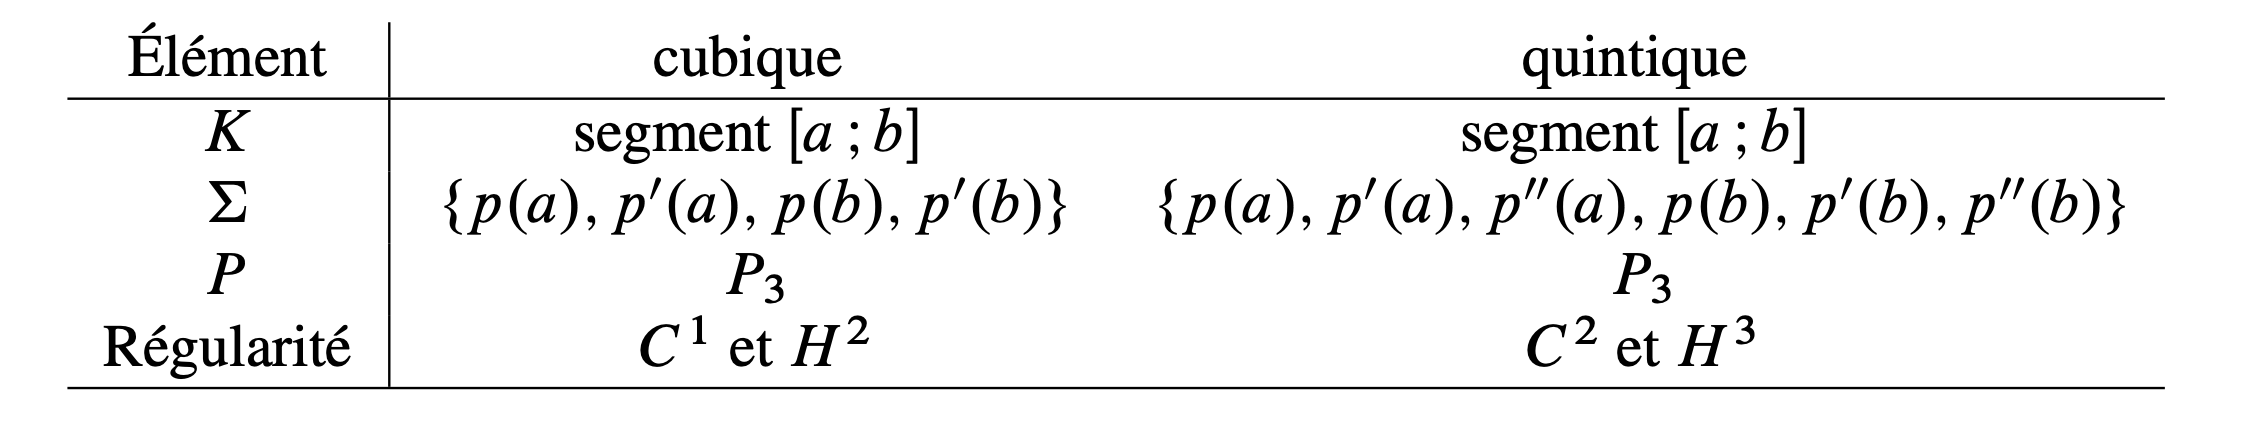
\includegraphics[scale=0.3]{hermite3-5.png} 
\end{center}
\begin{center}
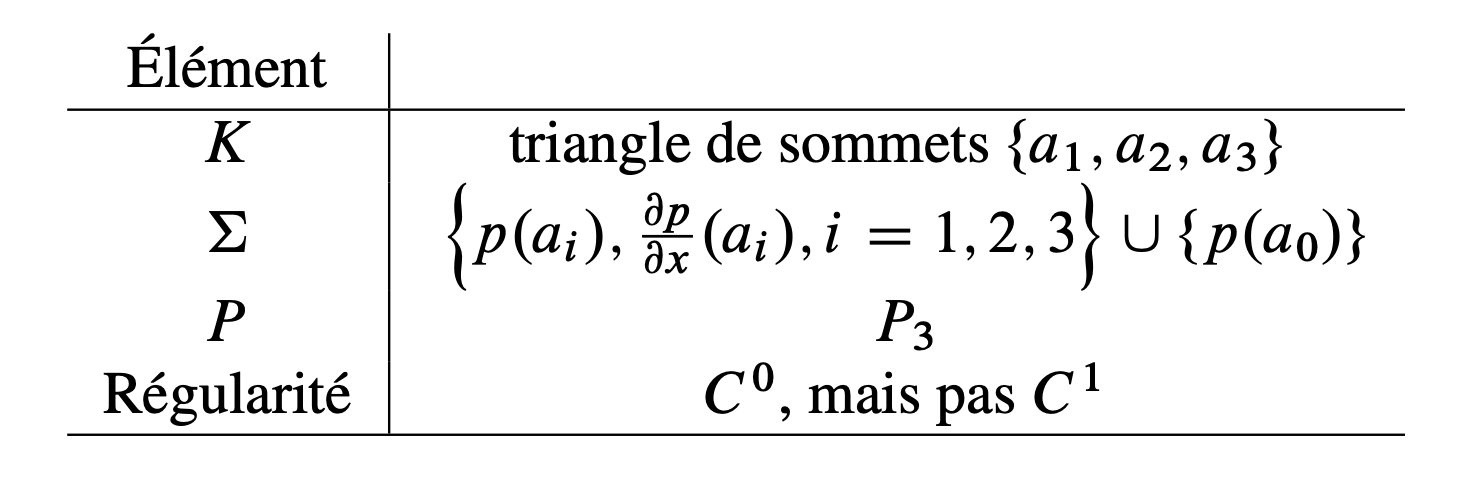
\includegraphics[scale=0.3]{hermiteTriangle1.png} 
\end{center}
\end{frame}
%%%%%%%%%%%%%%%%%%%%%%%%%%%%%%%%%%%%%%%
\begin{frame}
\frametitle{Élément triangle}


\begin{center}
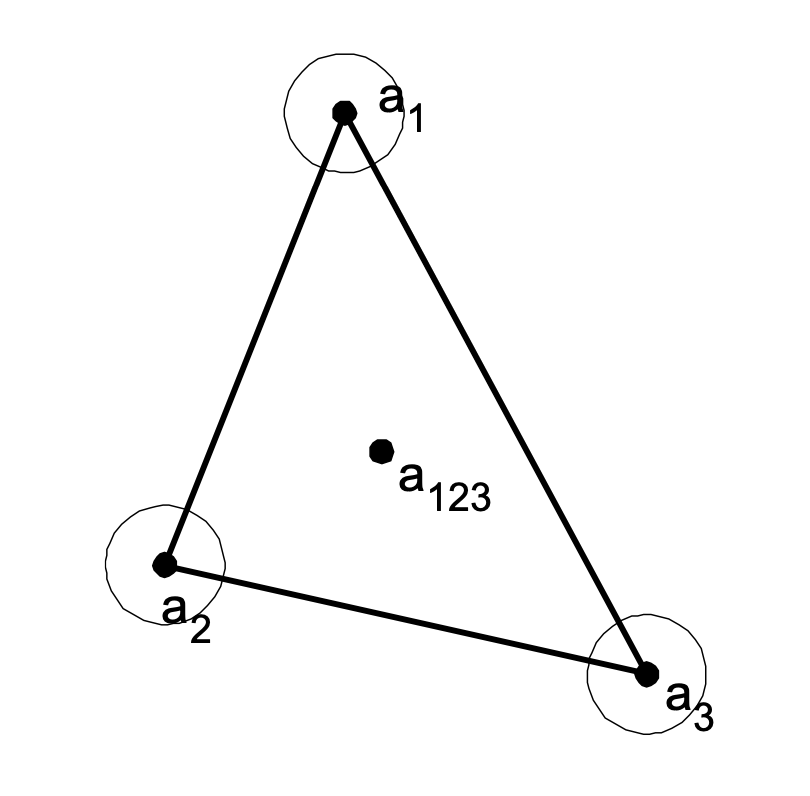
\includegraphics[scale=0.3]{hermiteTriangleUN.png} 
\end{center}
\begin{center}
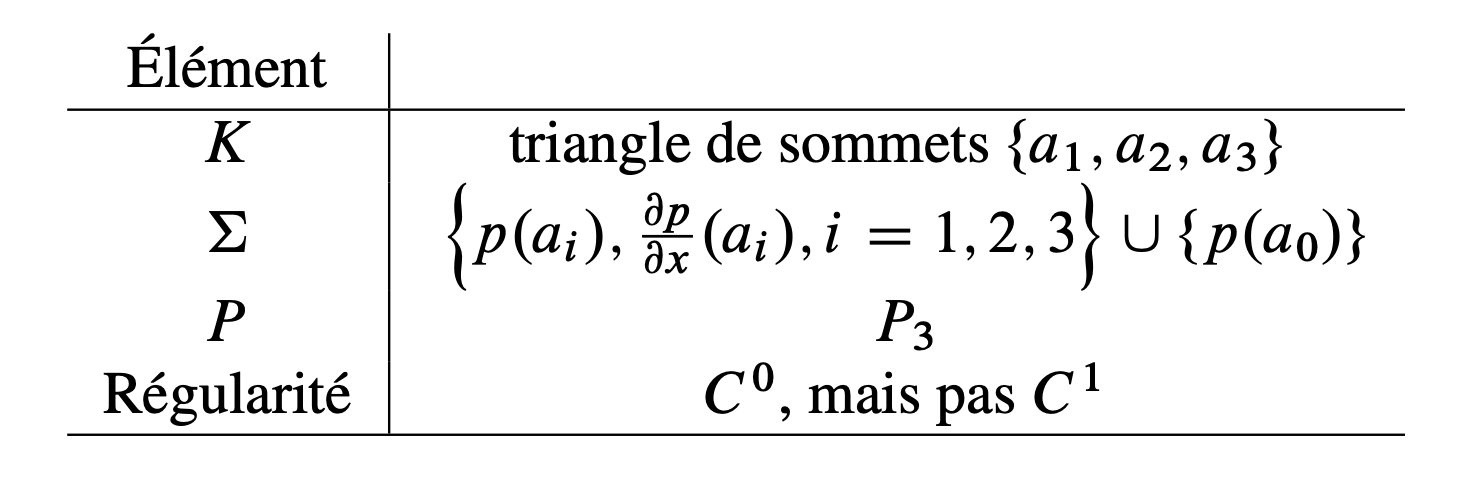
\includegraphics[scale=0.3]{hermiteTriangle1.png} 
\end{center}
\end{frame}
%%%%%%%%%%%%%%%%%%%%%%%%%%%%%%%%%%%%%%%
\begin{frame}
\frametitle{Éléments bidimensionnels}
\begin{center}
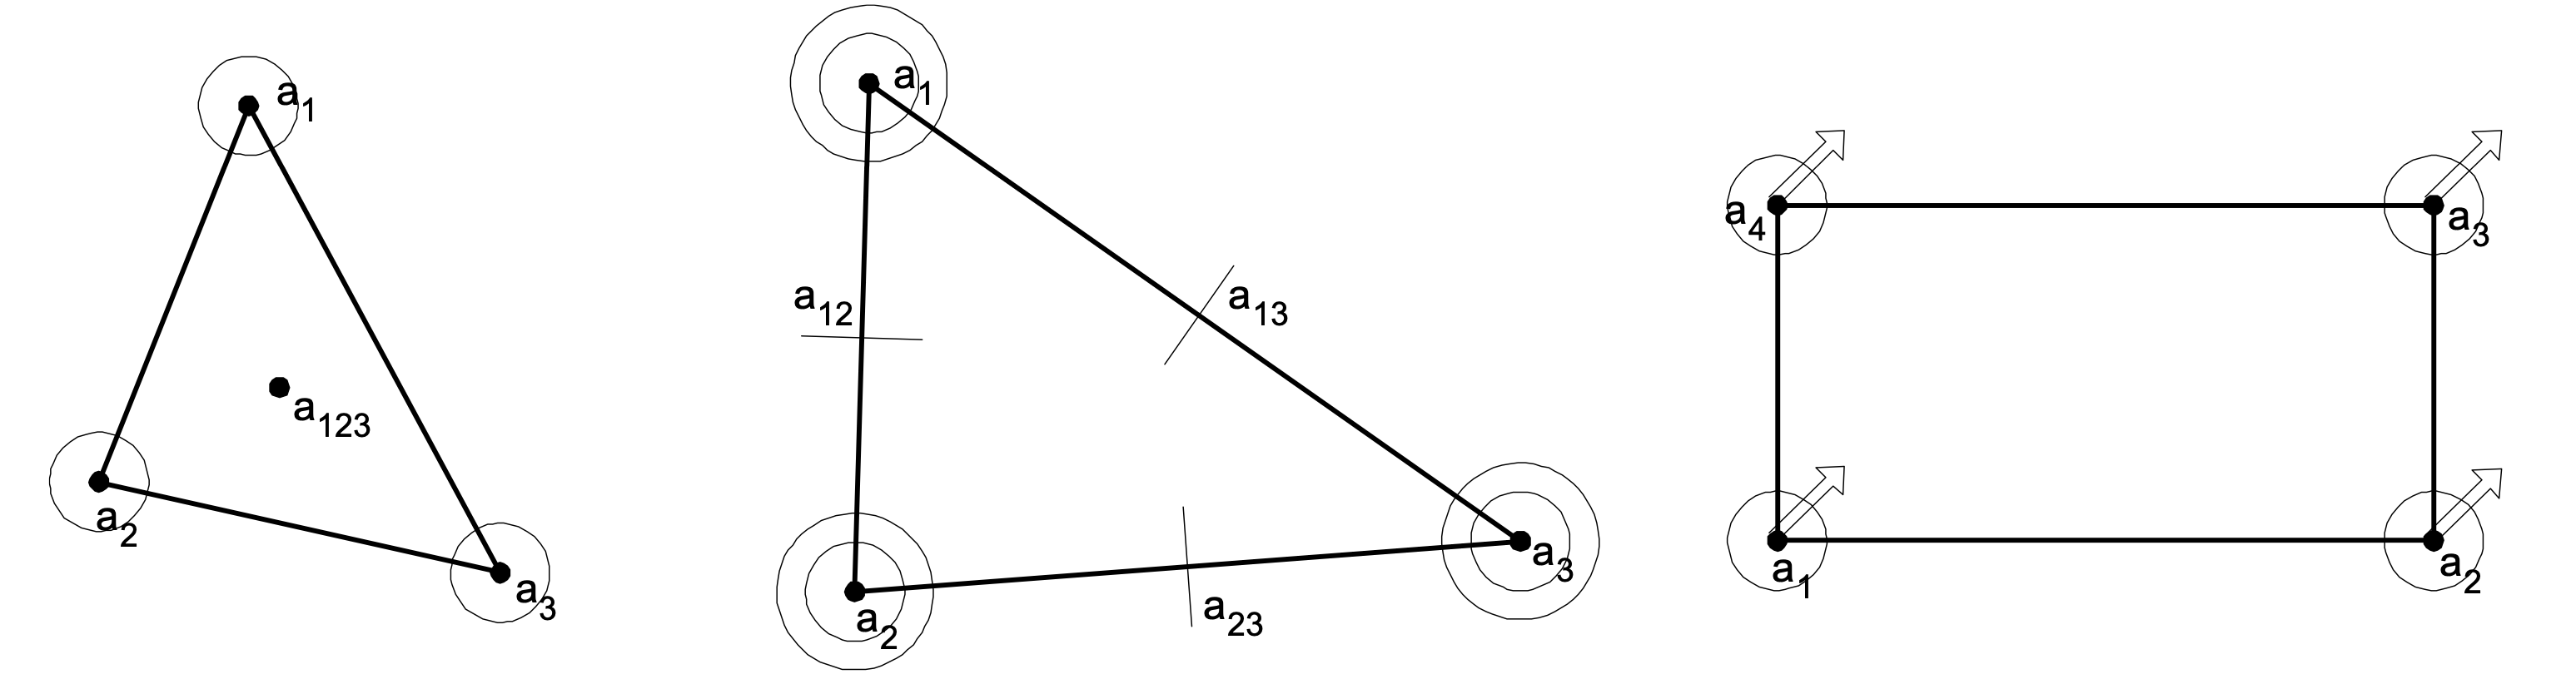
\includegraphics[scale=0.2]{elementsHermite.png} 
\end{center}
\begin{center}
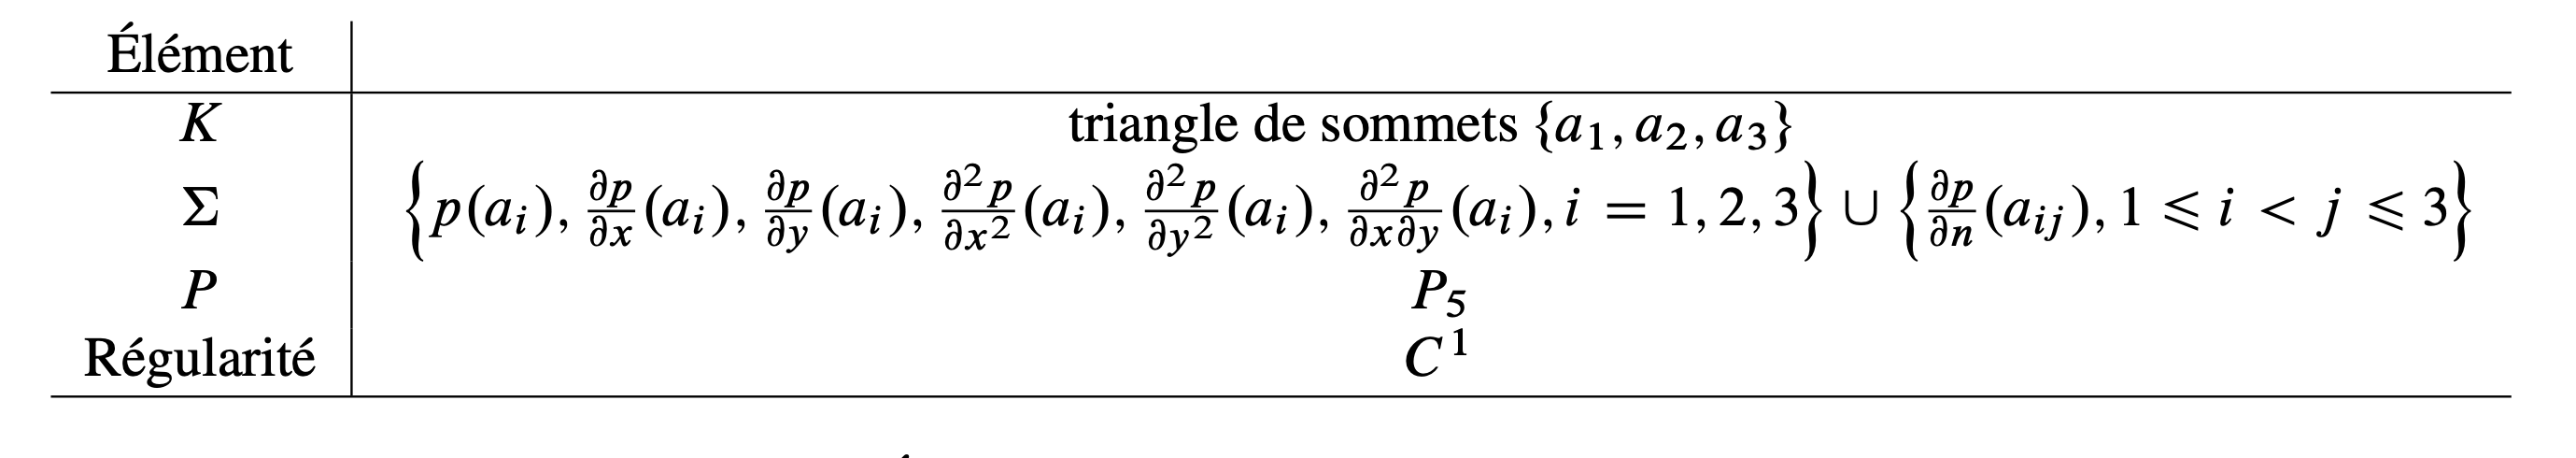
\includegraphics[scale=0.25]{hermiteBidim1.png} 
\end{center}
\begin{center}
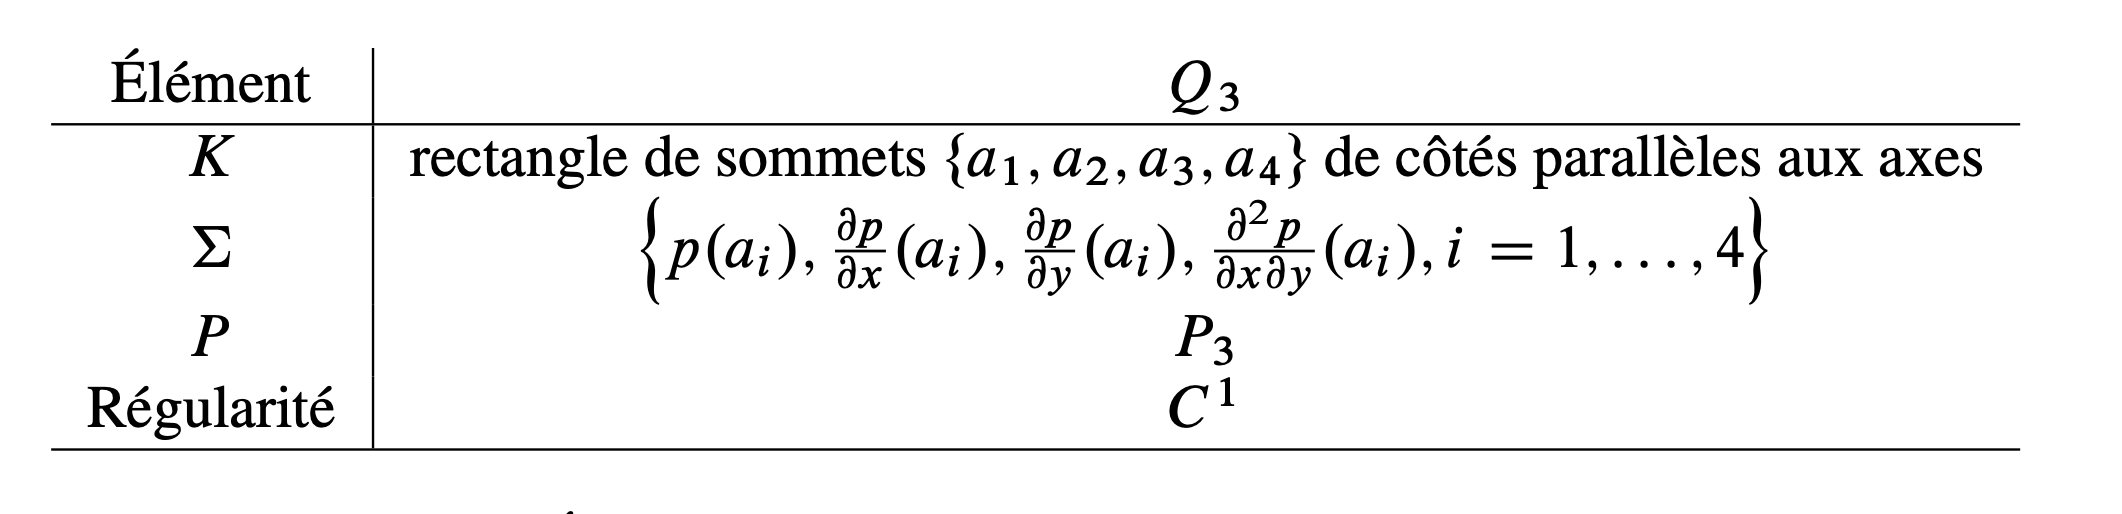
\includegraphics[scale=0.25]{hermiteBidim2.png} 
\end{center}

\end{frame}



\begin{frame}
\frametitle{Les fonctions de base}

\begin{itemize}
\item $\Phi_{i}(x)$ les fonctions de base associées aux valeurs nodales de la fonction $v_{i}$.
\item $\Psi_{i}(x)$ les fonctions de base associées aux valeurs nodales de la dérivée $(\frac{dv}{dx})_{i}$,
\end{itemize}


\begin{displaymath}
\Pi v (x)=\sum_{i=1}^{n}v_{i}\Phi_{i}(x)+\sum_{i=1}^{n}(\frac{dv}{dx})_{i}\Psi_{i}(x)\end{displaymath}

Sur un élément $[x_{1},x_{2}]$, cette approximation s'écrit:

\begin{displaymath}
v^{h}(x)=v_{1}\Phi_{1}(x)+(\frac{dv}{dx})_{1}\Psi_{1}(x)+v_{2}\Phi_{2}(x)+(\frac{dv}{dx})_{2}\Psi_{2}(x)\end{displaymath}

$\Phi_{i}$ et $\Psi_i$ vérifient les conditions:
\[\left\{\begin{array}{l}
\Phi_{i}(x_j)=\delta_{ij}\quad \Phi'_{i}(x_j)=0\\
\Psi_{i}(x_j)=0\quad \Psi'_{i}(x_j)=\delta_{ij}
\end{array} \right. \]
\end{frame}



\begin{frame}
\frametitle{Les fonctions de base}
\[\left\{\begin{array}{l}
\Phi_i(x) = \left[1-2(x-x_i)\lambda'_i(x_i)\right]\lambda^2_i(x) \\
\Psi_i(x) = (x-x_i)\lambda^2_i(x) 
\end{array}\right.
 \]
 \begin{itemize}
 \item élément de référence de longueur $h$:  $x_1=0$ et $x_2=h$, 
 \item $\lambda_1(x)=1-\frac{x}{h}$ et $\lambda_2(x)=\frac{x}{h}$. On pose $\xi= \frac{x}{h}$:
 \[\left\{\begin{array}{l}
\Phi_1(x) = (1+2\xi)(1-\xi)^2 \\
\Phi_2(x) = (3-2\xi)\xi^2 \\
\Psi_1(x) = h \xi(1-\xi)^2\\
\Psi_2(x) = h (\xi-1)\xi^2
\end{array}\right.
 \]
 \begin{center}
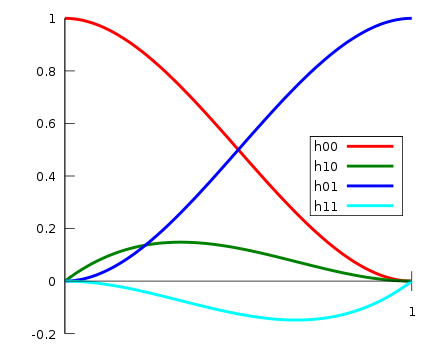
\includegraphics[scale=0.25]{HermiteBasis.png} 
\end{center}
 \end{itemize}

\end{frame}



%%%%%%%%%%%%%%%%%%%%%%%%%%%%%%%%%%%%%%%%%%%%%%%%%%%

\begin{frame}
\frametitle{Erreur d'interpolation}
Soit $(K,\mathbb{P},\Sigma)$ un élément fini $n$-simplexe ou $n$-palallélotope de type ($k$). On suppose
\[n\leq 3\quad \mbox{ et }\quad k\geq 1\]
Alors il existe une constante $C$ qui ne dépend que de $n$ et de $k$ telle que pour tout entier $m$, $0\leq m\leq k$, on a
\[\forall v\in H^{k+1}(K),\quad |v-\Pi v|_{m,k}\leq \frac{h_K^{k+1}}{\rho_K^m}|v|_{k+1,K}\]
\begin{center}
\begin{tikzpicture}
\draw [orange] (1,1) circle (1cm);
\draw (0,0) -- (0,2.655);
\draw (0,0) -- (5.2,0);
\draw [domain=0:5.2] plot(\x,-\x/2+2.6355);
\draw [olive,domain=0.1:5.35,<->] plot(\x,-\x/2+3);
\draw [olive,<->](0,1) -- (1,1);
 \draw[->] (0.5,0.8) node{$\rho$};
 \draw (2.5,2) node{$h$};
\end{tikzpicture}
\end{center}
 
\end{frame}
%%%%%%%%%%%%%%%%%%%%%%%%%%%%%%%%%%%%%%%%%%%%%%%%%%%


\begin{frame}
\frametitle{Intégration numérique}
\[a(\varphi_j,\varphi_i)=\sum_{l,m}^2\left(a_{lm}\sum_{K\in{\cal T}_h}\int_K\frac{\partial \varphi_j}{\partial x_m}\frac{\partial \varphi_i}{\partial x_l}\de x\right)\]
\begin{itemize}
\item Les fonctions de base appartiennent à $\mathbb{P}_k$ donc le produit $\frac{\partial \varphi_j}{\partial x_m}\frac{\partial \varphi_i}{\partial x_l}$ coïncide avec un polynôme de $\mathbb{P}_{2k-2}$.
\item Soit $F_K:\hat{x}\mapsto F_K(\hat{x})=B_K \hat{x}+b$ une bijection affine du triangle unité $\widehat{K}$ sur le triangle $K$;  det$(B_K)>0$. 
\begin{center}
\begin{tikzpicture}[domain=0:5,scale=0.35]
 \pgfmathsetmacro{\alpha}{0.05}
  \pgfmathsetmacro{\a}{0.5}
  \draw[->] (0,0) -- (5,0)  node[right] {$\xi$};
  \draw[->] (0,0) -- (0,5) node[left] {$\eta$};
  \draw (3,0)  node[above right] {$\scriptstyle  \widehat{a}_1$};
  \draw (0,3)  node[above right] {$\scriptstyle  \widehat{a}_2$};
  \draw (0,0)  node[above left] {$\scriptstyle  \widehat{a}_3$};
  \draw (0.8,1.5)  node {$\scriptstyle  \widehat{x}$};
  \draw (12.2,2.4)  node {$\scriptstyle  x$};
 \draw[->] (8,0) -- ++(7,0)  node[right] {$x$};
  \draw[->] (8,0) --++ (0,5) node[left] {$y$};
   \draw[blue,thick,fill=blue!30, fill opacity=0.6](10,2)-- ++(3,-1)-- ++(0,3)-- ++(-3,-2);

\path[fill=gray] (10,2) circle (1.0mm)node[left,below] {$\scriptstyle  a_3$};
\path[fill=gray] (13,1) circle (1.0mm)node[left,below] {$\scriptstyle  a_1$};
\path[fill=gray] (13,4) circle (1.0mm)node[right] {$\scriptstyle  a_2$};


\draw[fill=orange!30, fill opacity=0.6] (0,0) -- ++(3,0) -- ++(-3,3) -- ++(0,-3) ;
%\draw (2,-0.5)  node[below] {$\scriptstyle  \widehat{x} =\lambda_1\widehat{a}_1+\lambda_2\widehat{a}_2+\lambda_3\widehat{a}_3$};
%\draw (11,-0.5)  node[below] {$\scriptstyle  x =\lambda_1 a_1+\lambda_2 a_2+\lambda_3 a_3$};
 \draw [->, >=latex,olive] (1,1.5) arc (120:70:13) ;
\end{tikzpicture}

\end{center}
Alors on a pour toute fonction $\varphi=\widehat{\varphi}\circ F_K$ continue sur $K$:
\[\int_K\psi(x)\de x =\mbox{dét}(B_K)\int_{\widehat{K}}\widehat{\psi}(\hat{x})\de \hat{x}\]
\end{itemize}




\end{frame}
%%%%%%%%%%%%%%%%%%%%%%%%%%%%%%%%%%%%%%%%%%%%%%%%%%%

\begin{frame}
\frametitle{Intégration de $a(\varphi_j,\varphi_i)$}
On a 
\[\mbox{dét}(B_K)=\frac{\mbox{mes}(K)}{\mbox{mes}(\widehat{K})}=2\mbox{mes}(K)\]
On prend $\psi=\frac{\partial \varphi_j}{\partial x_m}\frac{\partial \varphi_i}{\partial x_l}\in \mathbb{P}_{2k-2}$. On se ramène à $\widehat{\psi}\in \mathbb{P}_{2k-2}$ sur le triangle unité. Or pour tout monôme $\hat{x}_1^{k_1}\hat{x}_2^{k_2}$:
\[\int_{\widehat{K}}\hat{x}_1^{k_1}\hat{x}_2^{k_2}\de \hat{x}=\frac{k_1!k_2!}{(k_1+k_2+2)!}\]
plus généralement
\[\int_{\widehat{K}}\hat{x}_1^{k_1}\hat{x}_2^{k_2}(1-\hat{x}_1-\hat{x}_2)^{k_3}\de \hat{x}=\frac{k_1!k_2!k_3!}{(k_1+k_2+k_3+2)!}\]
En coordonnées barycentriques
\[\int_{\widehat{K}}\lambda_1^{k_1}\lambda_2^{k_2}\lambda_3^{k_3}\de \hat{x}=2\mbox{mes}(K)\frac{k_1!k_2!k_3!}{(k_1+k_2+k_3+2)!}\]

\end{frame}
%%%%%%%%%%%%%%%%%%%%%%%%%%%%%%%%%%%%%%%%%%%%%%%%%%%

\begin{frame}
\frametitle{Intégration de $\ell(\varphi_i)$}
\[\ell(\varphi_i)=\sum_{K\in{\cal T}_h}\int_K f \varphi_i\,\de x\]
Formule de quadrature: $\int_K f \psi(x)\,\de x\simeq \sum_{i=1}^N\omega_{l,K}\psi(b_{i,K})$
\begin{itemize}
\item $k=0$: 
\[\int_K \psi(x)\,\de x\simeq \mbox{mes}(K) \psi(a_{0,K})\]
\item $k=1$: 
\[\int_K \psi(x)\,\de x\simeq \frac 13\mbox{mes}(K) \sum_{i=1}^3\psi(a_{i,K})\]
\item $k=2$: 
\[\int_K \psi(x)\,\de x\simeq \frac 13\mbox{mes}(K) \sum_{i=4}^6\psi(a_{i,K})\]
\end{itemize}
\end{frame}
%%%%%%%%%%%%%%%%%%%%%%%%%%%%%%%%%%%%%%%%%%%%%%%%%%%
\begin{frame}
\frametitle{Intégration de $\ell(\varphi_i)$}
\[\ell(\varphi_i)=\sum_{K\in{\cal T}_h}\int_K f \varphi_i\,\de x\]
Formule de quadrature: $\int_K f \psi(x)\,\de x\simeq \sum_{i=1}^N\omega_{l,K}\psi(b_{i,K})$
\begin{itemize}
\item $k=0$: 
\[\int_K \psi(x)\,\de x\simeq \mbox{mes}(K) \psi(a_{0,K})\]
\item $k=1$: 
\[\int_K \psi(x)\,\de x\simeq \frac 13\mbox{mes}(K) \sum_{i=1}^3\psi(a_{i,K})\]
\item $k=2$: 
\[\int_K \psi(x)\,\de x\simeq \frac 13\mbox{mes}(K) \sum_{i=4}^6\psi(a_{i,K})\]
\end{itemize}
\end{frame}
%%%%%%%%%%%%%%%%%%%%%%%%%%%%%%%%%%%%%%%%%%%%%%%%%%%

\begin{frame}
\frametitle{Maillage }
\begin{itemize}
\item Un maillage (ou triangulation) de $\Omega$ est la donnée de $N_{el}$ triangles
$\{K_1, . . .,K_{Nel}\}$ (fermés par convention) formant une partition de $\Omega$.
\[\overline{\Omega}=\bigcup_{i=1}^{N_{el}}K_i,\quad \mathring{K_i}\cap \mathring{K_j}=\emptyset,\; \forall i\neq j\]

\item Le maillage est admissible si pour tout $K_i \neq K_j$, l'ensemble $K_i \cap K_j$ est
\begin{enumerate}
\item soit vide
\item soit un sommet commun $K_i$ et $K_j$
\item soit une arête commune $K_i$ et $K_j$
\end{enumerate}
\begin{center}
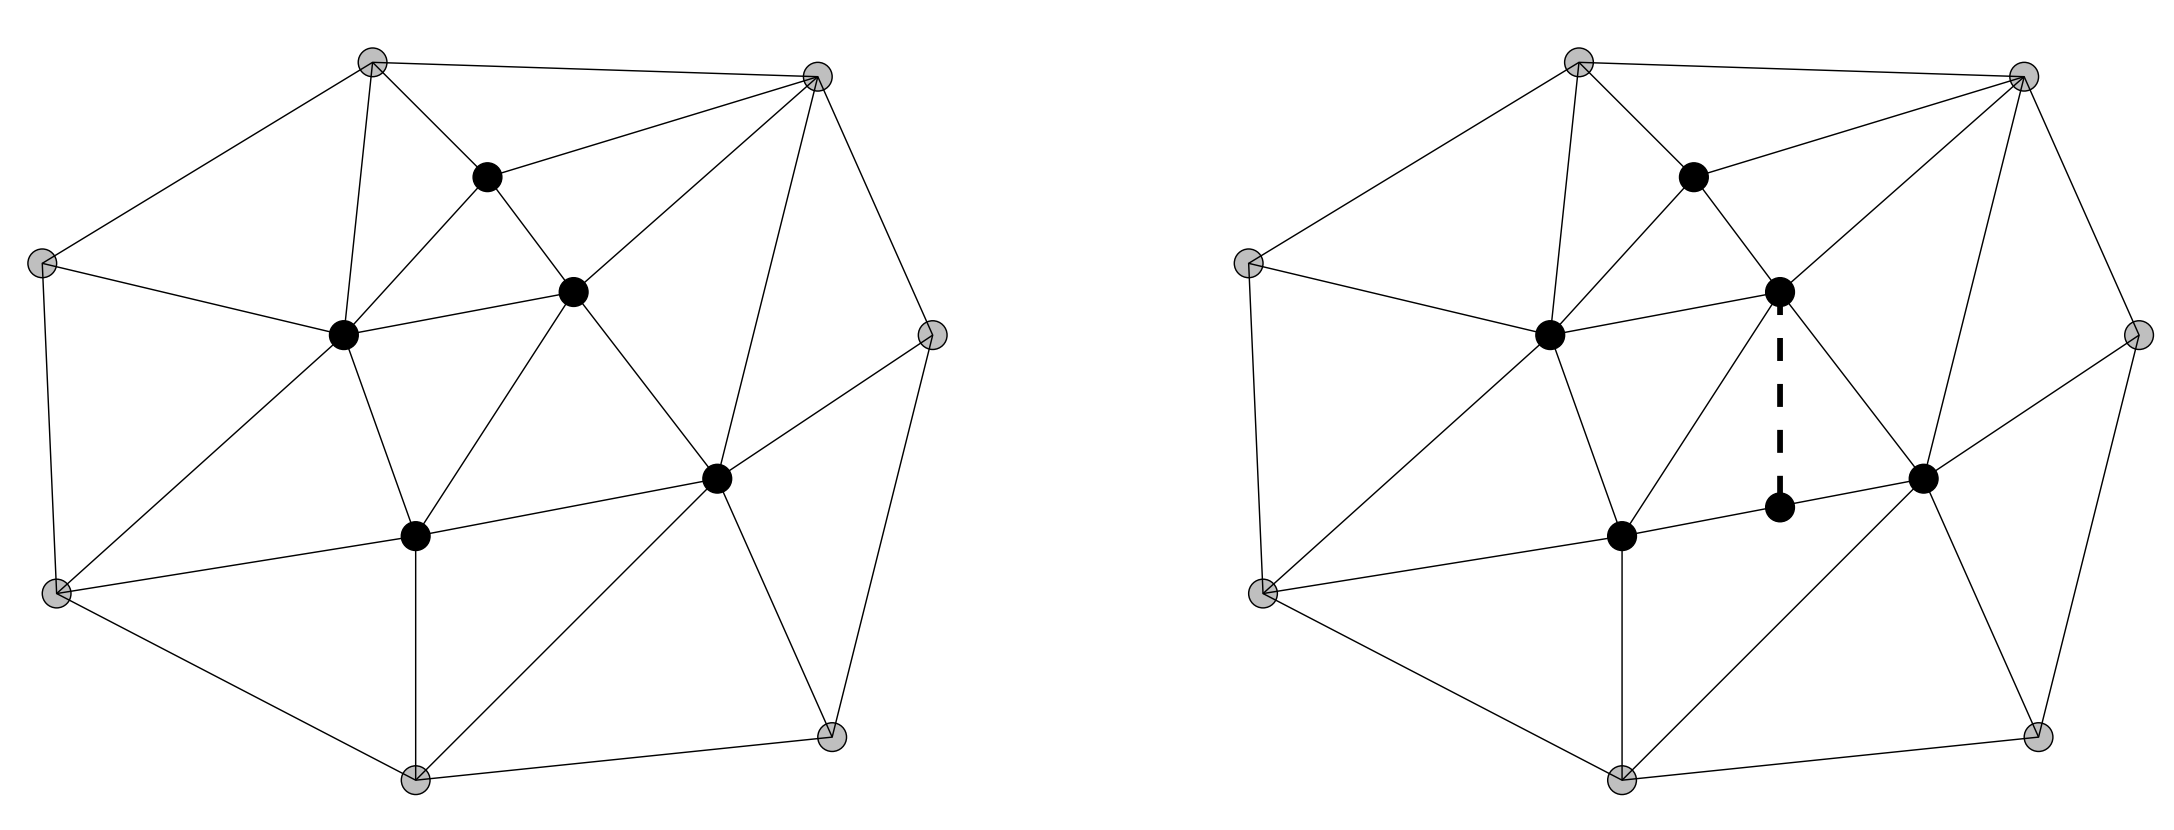
\includegraphics[scale=0.25]{maillage01.png} 
\end{center}
\end{itemize}
\end{frame}
%%%%%%%%%%%%%%%%%%%%%%%%%%%%%%%%%%%%%%%%%%%%%%%%%%%

\begin{frame}
\frametitle{Relations d'Euler}
\begin{itemize}
\item On note
\begin{itemize}
\item $N_{el}$ le nombre d'éléments
\item $N_{ar}$ le nombre d'arêtes
\item $N_{so}^{int}$  le nombre de sommets intérieurs
\item $N_{so}^{ext}$  le nombre de sommets extérieurs
\item $N_{so}=N_{so}^{int}+N_{so}^{ext}$  le nombre total de sommets
\end{itemize}

\item Pour tout maillage admissible, on a (relations d'Euler)
\[N_{el}=N_{so}+N_{so}^{int}-2(1-J)\qquad N_{ar}=2N_{so}+N_{so}^{int}-3\]
($J$: nombre de trous dans $\Omega$)
\item Dans la limite pratique $N_{so}^{ext}<< N_{so}$ et $N_{so}^{int}\sim N_{so}$, il vient
\[N_{el}\sim 2N_{so}^{int} \qquad N_{ar}\sim 3N_{so}^{int} \]
\end{itemize}
\end{frame}
%%%%%%%%%%%%%%%%%%%%%%%%%%%%%%%%%%%%%%%%%%%%%%%%%%%

\begin{frame}
\frametitle{Échelles de longueur (1)}
\begin{itemize}
\item On introduit pour chaque maille $K_i$ deux échelles de longueur
\begin{itemize}
\item son diamètre $h_i$
\item le diamètre de son cercle inscrit $\rho_i$
\end{itemize}

\item On a $h_i/\rho_i \geq 1$  et $h_i/\rho_i >> 1$ lorsque le triangle $K_i$ est très  aplati
\begin{center}
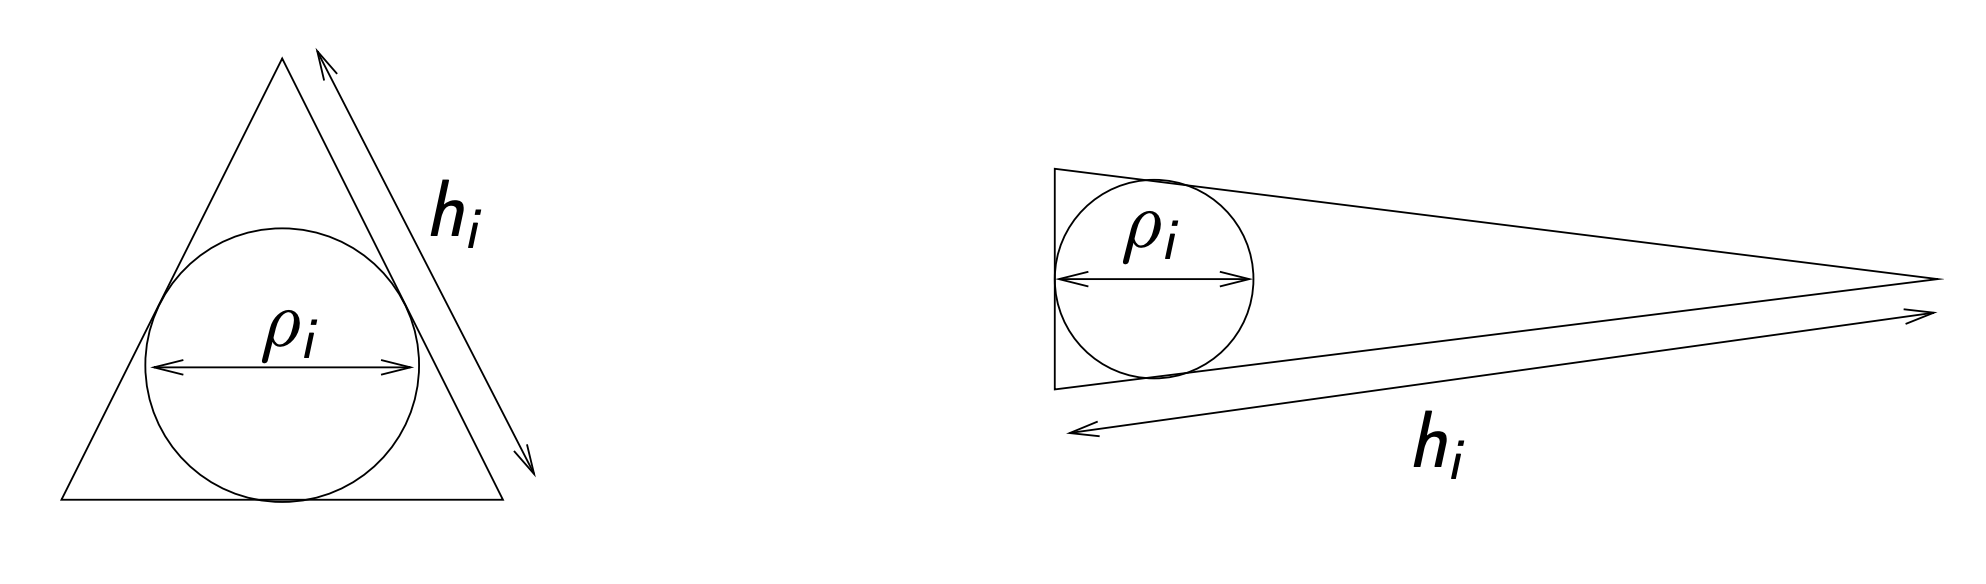
\includegraphics[scale=0.25]{maillage02.png} 
\end{center}
\item On a $h_i/\rho_i \leq \frac{2}{\sin\theta_i}$ $\theta_i$ est le plus petit angle du triangle $K_i$
\end{itemize}
\end{frame}
%%%%%%%%%%%%%%%%%%%%%%%%%%%%%%%%%%%%%%%%%%%%%%%%%%%

\begin{frame}
\frametitle{Échelles de longueur (2)}
\begin{itemize}
\item On introduit pour chaque maille $K_i$ deux échelles de longueur
\begin{itemize}
\item son diamètre $h_i$
\item le diamètre de son cercle inscrit $\rho_i$
\end{itemize}

\item On a $h_i/\rho_i \geq 1$  et $h_i/\rho_i >> 1$ lorsque le triangle $K_i$ est très  aplati
\begin{center}
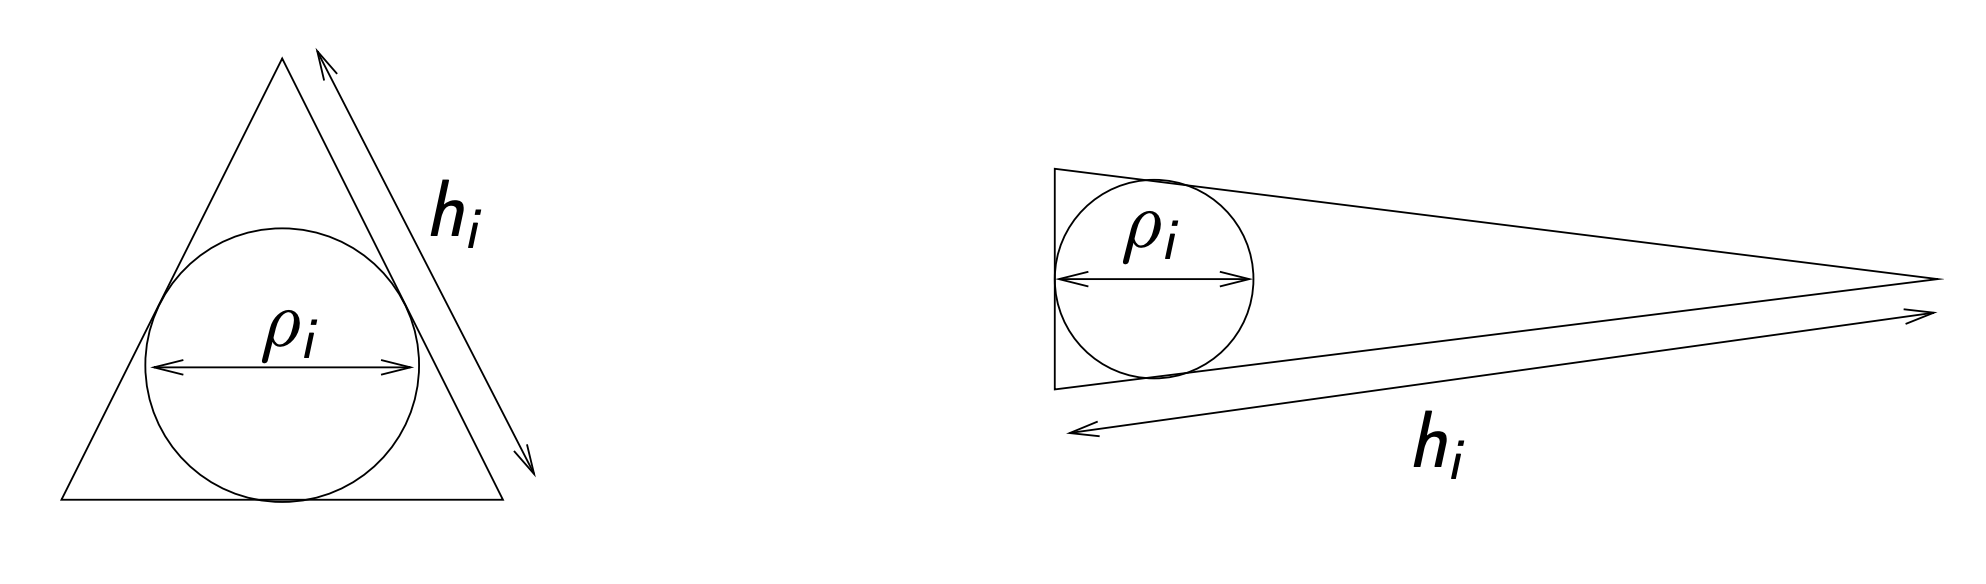
\includegraphics[scale=0.25]{maillage02.png} 
\end{center}
\item On a $h_i/\rho_i \leq \frac{2}{\sin\theta_i}$ $\theta_i$ est le plus petit angle du triangle $K_i$
\end{itemize}
\end{frame}
%%%%%%%%%%%%%%%%%%%%%%%%%%%%%%%%%%%%%%%%%%%%%%%%%%%


\begin{frame}
\frametitle{Échelles de longueur (2)}
\begin{itemize}
\item Pour un maillage $\{K_1 . . .,K_{N_{el}}\}$, on introduit les paramètres globaux
\[h=\max_{1\leq i\leq N_{el}} h_i\qquad \sigma =\max_{1\leq i\leq N_{el}} \frac{h_i}{\rho_i}\]
\item Pour un maillage quasi-uniforme, $\sigma\gtrsim  1$ et $h_i \sim h$
\item Pour un maillage quasi-uniforme, on a $h \sim (N_{el})^ {-1/2}$
\begin{enumerate}
\item en 1D, $h \sim (N_{el})^{-1}$
\item en dimension $d$, $h \sim (N_{el})^{-1/d}$
\item à $h$ fixé, plus $d$ est grand, plus il faut de mailles!
\end{enumerate}
\item Exemple de maillage avec raffinement local

\begin{center}
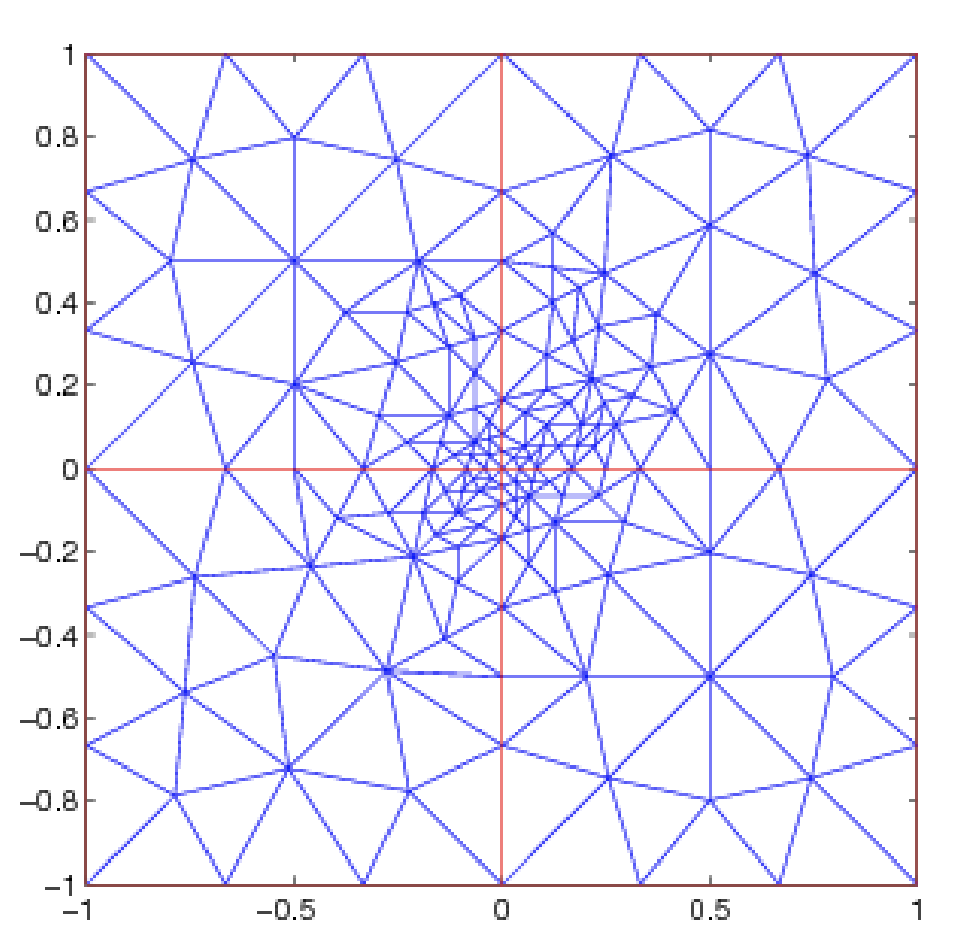
\includegraphics[scale=0.22]{maillage03.png} 
\end{center}
\item On a $h_i/\rho_i \leq \frac{2}{\sin\theta_i}$ $\theta_i$ est le plus petit angle du triangle $K_i$
\end{itemize}
\end{frame}
%%%%%%%%%%%%%%%%%%%%%%%%%%%%%%%%%%%%%%%%%%%%%%%%%%%

\end{document}






\begin{frame}
\frametitle{Maillage triangulaire (ou triangulation)}
 Un maillage est conforme s’il suit les quelques règles simples suivantes. Une illustration est proposée sur la figure 3.
— L’union des 𝑁𝑡 triangles doit couvrir Ω sans le dépasser : Ω = ⋃︀𝑁𝑡 𝐾𝑝. 𝑝=1
— L’intersection de deux triangles est soit vide, soit une arête commune complète à chacun des deux triangles, soit un sommet de chacun des deux triangles.
— Une arête d’un triangle est soit une arête (complète) d’un autre triangle, soit une partie de Γ, auquel cas ce segment est complètement inclus soit dans Γ𝐷 soit dans Γ𝑁 (il n’y a pas d’arête appartenant à la fois à Γ𝐷 et à Γ𝑁 ).
\end{itemize}
\end{frame}
%%%%%%%%%%%%%%%%%%%%%%%%%%%%%%%%%%%%%%%%%%%%%%%%%%%

\end{document}


